\documentclass[12pt]{article}

\usepackage{amssymb,amsmath,amsfonts,eurosym,geometry,ulem,graphicx,caption,color,setspace,sectsty,comment,footmisc,caption,natbib,pdflscape,subfigure,array,hyperref}
\usepackage{xcolor} 
\definecolor{lightblue}{RGB}{100,149,237}
\usepackage{longtable} 
\usepackage{amssymb}
\usepackage{url}
\usepackage[table,xcdraw]{xcolor}
\usepackage{xcolor}
\usepackage{graphicx}
\usepackage{enumerate}
\usepackage{amsmath}
% \usepackage{amsthm}	
\usepackage{amsfonts, amssymb, float, placeins, tabularx, array, longtable, booktabs, listings} 
\usepackage{natbib}
\usepackage{threeparttable}
\usepackage{graphicx}
\usepackage{subcaption}
\normalem

\onehalfspacing
\newtheorem{theorem}{Theorem}
\newtheorem{corollary}[theorem]{Corollary}
\newtheorem{proposition}{Proposition}
\newenvironment{proof}[1][Proof]{\noindent\textbf{#1.} }{\ \rule{0.5em}{0.5em}}

\newtheorem{hyp}{Hypothesis}
\newtheorem{subhyp}{Hypothesis}[hyp]
\renewcommand{\thesubhyp}{\thehyp\alph{subhyp}}

\newcommand{\red}[1]{{\color{red} #1}}
\newcommand{\blue}[1]{{\color{blue} #1}}

\newcolumntype{L}[1]{>{\raggedright\let\newline\\arraybackslash\hspace{0pt}}m{#1}}
\newcolumntype{C}[1]{>{\centering\let\newline\\arraybackslash\hspace{0pt}}m{#1}}
\newcolumntype{R}[1]{>{\raggedleft\let\newline\\arraybackslash\hspace{0pt}}m{#1}}

\geometry{left=1.0in,right=1.0in,top=1.0in,bottom=1.0in}

\begin{document}

\begin{titlepage}
\title{The Effect of Cutting Renewal Road Tax Levies on House Values,  Wages, and Employment \thanks{Acknowledgements: We are grateful for comments from CK Tang, Guoyang Yang, Dan Boles, Eunjee Kwon, Gary Painter, Olivier Parent, Jeffrey Mills, Nayoung Lee, Matias Cattaneo, and Chris Bollinger, to CoreLogic® for leasing us the housing dataset, and to the Ohio Department of Jobs and Family Services (ODJFS) for providing us access to establishment-level employment data.}}
\author{David Brasington \thanks{Professor, University of Cincinnati} \and Saani Rawat \thanks{PhD Student, University of Cincinnati}}
\date{\today}
\maketitle

\noindent
\begin{center}
\textbf{\href{https://example.com/latest-draft}{\textcolor{lightblue}{Please click here for the latest draft.}}}
\end{center}

\begin{abstract}
\noindent     We investigate the economic impact of cutting road maintenance spending in Ohio. Using a regression discontinuity design, we analyze city-level votes to renew road maintenance tax funding, which typically represents about 34\% of road funding. We compare housing sale prices, wages, and employment between similar cities that narrowly pass or fail road tax levies. Cities that cut road maintenance spending suffer an average decrease in housing prices of \$20,729 (12\%) relative to cities that renewed funding. High-poverty cities that cut road spending have 11\% lower levels of employment and 17.8\% lower wages than similar cities that maintained their spending. \\
\vspace{0in}\\
\noindent\textbf{Keywords:} Road Maintenance, Local Taxation, Housing values, Employment, Wage \\
\vspace{0in}\\
\noindent\textbf{JEL Codes:} R42, H71, J31, R11, R21 \\

\bigskip
\end{abstract}
\setcounter{page}{0}
\thispagestyle{empty}
\end{titlepage}
\pagebreak \newpage




\doublespacing


\section{Introduction} \label{sec:introduction}

Roads are an important form of infrastructure investment that affect firms’ production functions and people’s commuting costs. Many studies examine the importance of roads and how they affect residents' daily lives (\Citeauthor{currier2023} \citeyear{currier2023}; \Citeauthor{adukia2020} \citeyear{adukia2020}, \Citeauthor{banerjee2020} \citeyear{banerjee2020}; \Citeauthor{banerjee2020} \citeyear{banerjee2020}, \Citeauthor{banerjee2020} \citeyear{banerjee2020}). Some papers emphasize that building new roads increases employment and entry of new firms \citep{gibbons2019new}, thereby increasing economic activity. Other papers point out the potential for worse outcomes in the form of increased inequality between the rich and the poor \citep{hettige2006} and an exodus of workers seeking access to larger labor markets \citep{asher2020}.  
 
In this paper, we highlight the importance of maintaining road spending for cities in Ohio. We collect data on more than 3,000 road-tax levy renewal elections conducted within different county subdivisions (referred to as “cities”)  in Ohio. Using regression discontinuity design, we examine how cuts in maintenance spending influence key economic outcomes, focusing on cities where voting results were narrowly decided. Our results reveal that cutting maintenance spending by 34\% decreases house prices by \$20,729, with the effect starting four years after the vote and persisting through nine years after the vote. The \$20,729 discount represents about 12 percent of house value over the decade.  The delayed effect is consistent with the time it might take for roads to deteriorate noticeably.  We further find that these price effects are more pronounced in urban areas, where house prices fall by approximately \$25,825 on average, compared to no significant changes in rural areas. We also observe that higher-priced homes experience larger reductions in value relative to lower-priced homes, indicating a heterogeneous impact across different quantiles of home prices. On the other hand, we find little evidence for any overall change in wages or employment as a result of the decreased road maintenance spending for our full sample.  We do find, however, an effect on employment and wages in high-poverty cities.  Cities above the 75th percentile of poverty that cut road maintenance taxes have 17.8\% lower wages than otherwise similar cities that barely renew road tax levies.  High-poverty cities that cut road tax levies also lose about 11\% more jobs than those that successfully renew maintenance spending.  We speculate that the amenity value of attractive roads, changes in business productivity, and compensating wage differentials are probably responsible for the results, rather than changes in traffic noise or crime rates.

Perhaps the study most related to ours is \cite{asher2020}, which studies the impact of new roads on villages in India. Like our study, its identification strategy is regression discontinuity, although ours is sharp rather than the fuzzy form.  It argues the main obstacle to identification in prior studies is that the placement of new roads is usually correlated with economic (or political) characteristics rather than exogenous.  Its findings suggest this is a serious problem with the literature because, unlike prior studies, it finds no strong link between economic growth and new road placement, suggesting that the estimates of previous studies that find a link are driven by road placement in villages that are already growing. \cite{asher2020} touts its use of village-level rather than regional-level data.  We, too, look at economic outcomes at the level of village, city, and township, the most local levels of government.  A surprising finding of \cite{asher2020} is that investment in transportation infrastructure does not affect village incomes, assets, or agricultural output.  Its measure of assets is a village-level average of a series of binary indicators of ownership of a variety of assets, along with separate regressions for the presence of a ‘solid house’, refrigerator, and phone; whereas we study the effect of transportation spending on wages, employment, and housing sale prices.  Of course, our use of a developed geography contrasts with rural villages in India.  Our efforts to achieve identification focus on the maintenance of existing roads, which avoids the endogeneity of the placement of new roads.


\section{Literature Review} \label{sec:literature}

{\bf Related Literature.} Perhaps the study most related to ours is \cite{asher2020}, which studies the impact of new roads on villages in India. Like our study, its identification strategy is regression discontinuity, although ours is sharp rather than the fuzzy form.  It argues the main obstacle to identification in prior studies is that the placement of new roads is usually correlated with economic (or political) characteristics rather than exogenous. Its findings suggest this is a serious problem with the literature because, unlike prior studies, it finds no strong link between economic growth and new road placement, suggesting that the estimates of previous studies that find a link are driven by road placement in villages that are already growing. \cite{asher2020} touts its use of village-level rather than regional-level data.  We, too, look at economic outcomes at the level of village, city, and township, the most local levels of government.  A surprising finding of \cite{asher2020} is that investment in transportation infrastructure does not affect village incomes, assets, or agricultural output.  Its measure of assets is a village-level average of a series of binary indicators of ownership of a variety of assets, along with separate regressions for the presence of a ‘solid house’, refrigerator, and phone; whereas we study the effect of local road tax cuts on housing sale prices.  Of course, our use of a developed geography contrasts with rural villages in India.  Our efforts to achieve identification focus on the maintenance of existing roads, which avoids the endogeneity of the placement of new roads.

Another study related to ours is \cite{cellini2010value}, which studies the effect of new capital projects for schools, funded via new local bond issues and raised by referendums. Both our study and \cite{cellini2010value} employ a dynamic regression discontinuity design and analyze changes in regional property values. Moreover, both papers rely on broadly similar identification strategies and assignment mechanisms: in each case, votes in favor of or against a local referendum serves as the source of exogenous variation. Despite these similarities, a few key distinctions stand out. First, \cite{cellini2010value} draws on all observations in their sample, while we limit our analysis to the optimal bandwidth around the 50\% vote-share cutoff, even after using flexible controls. Second, \cite{cellini2010value} implements a fuzzy regression discontinuity approach, whereas ours is sharp. Lastly, we focus on the Intent-to-Treat (ITT) estimator, which analyzes the effect of an election on outcomes without controlling for the results of subsequent elections. The ITT estimator suits our setting given the independence of renewal referendums characterized by exogenous timing (more details in Section \ref{sec:empirical}). As \cite{cellini2010value} show, when elections are independent, the ITT estimator is equal to the Treatment on the Treated (TOT) estimator. 

% We highlight a substantial literature studying the effect of transportation infrastructure on house prices. \cite{hoogendoorn2019house} studies the effect of the opening of a tunnel on house prices in the Netherlands, noting that prior research studying transportation infrastructure in developed geographies suffers from reverse causality.  It argues that the opening of the Westerscheldtunnel is a fairly exogenous event, with natural borders that prevent contamination of results by the surrounding environment. \cite{hoogendoorn2019house} finds half the capitalized value of the tunnel occurs more than a year before the tunnel opens and argues that the exogeneity of the opening of the tunnel, along with hedonic controls, time trends and postcode fixed effects, identifies its estimates. Our data, too, is for a developed nation. One novelty of our study is how ordinary the events are that we study. While the opening of a new tunnel is important, it is rare.  Votes to renew infrastructure spending are common events in many local governments in the United States, and the quantity of road maintenance spending is regularly chosen by governments around the world, if not by voting then directly by bureaucrats. It is therefore also important to study the effects of road maintenance spending on house prices. 

We highlight a substantial literature studying the effect of transportation infrastructure on house prices. \cite{hoogendoorn2019house} studies the effect of the opening of a tunnel on house prices in the Netherlands, noting that prior research on transportation infrastructure in developed regions often suffers from reverse causality. It argues that the opening of the Westerscheldtunnel is a fairly exogenous event, with natural borders that prevent contamination of results by the surrounding environment. \cite{hoogendoorn2019house} finds that half the capitalized value of the tunnel occurs more than a year before the tunnel opens and argues that the exogeneity of the tunnel's opening, along with hedonic controls, time trends, and postcode fixed effects, identifies its estimates. Our data also pertains to a developed nation. One novelty of our study is how ordinary the events are that we study. While the opening of a new tunnel is significant, it is rare. Votes to renew infrastructure spending are common events in many local governments in the United States, and the amount of road maintenance spending is regularly determined by governments worldwide, either through voting or directly by bureaucrats. It is therefore important to study the effects of road maintenance spending on house prices.

\cite{li2016wheels} studies the overall effect on apartment prices of new subway lines in Beijing, but the estimates may represent the net effect of competing factors. \cite{gibbons2005valuing}, studying the construction of new rail stations for the London underground and light rail services, notes that the effect on house prices captures the net effect of better access, increased crime, and increased noise pollution. \cite{levkovich2016effects} looks at the effect of highway development on house prices in the Netherlands. It separates out accessibility effects from noise pollution and increased traffic effects by looking at different neighborhoods near the highway development. Its repeat sales difference in differences model finds increased house prices from anticipation effects \citep{kohlhase1991impact}. \cite{beenstock2016hedonic} also finds anticipation effects for house prices (but not new construction) for the development of a highway across Israel. 

{\bf Contribution.} Our paper contributes to the literature on three main fronts. First, we establish a new dataset that allows us to study how changes in local taxes affect local infrastructure maintenance and neighborhood house prices.  The votes on road maintenance taxes are matched with auditor data on road maintenance spending by Ohio cities, and property sale prices from CoreLogic. Our data also includes images of roads from Google Street Views API before and after cities vote to cut road maintenance. We train an artificial intelligence model to measure road attractiveness to see if cutting road taxes causes a decline in the physical appearance of roads.  

Second, we focus on long-term effects of reduced road taxes funded mainly via property taxes, and observe statistically significant decline in house prices occurring after four years and persisting in later years. This delayed effect highlights how the consequences of road tax cuts are not immediate but gradually accumulate as funding is reduced and roads deteriorate. Our research also identifies heterogeneous impacts, showing that urban areas and higher-priced houses suffer more pronounced price declines. By focusing on distributional effects, the study adds nuance to the understanding of how infrastructure maintenance affects local housing markets.

Third, while much of the literature focuses on new infrastructure development and expansion in developing nations, we study infrastructure maintenance in a developed economy.  Focusing on existing roads mitigates an important source of identification problems. Our approach provides insights that are more relevant for policymakers in advanced economies, where road infrastructure is well established but requires continuous upkeep. 

{\bf Roadmap.} The rest of the paper is organized as follows. Section \ref{sec:data} provides background information on the data and provides information about the variables used in the study. Section \ref{sec:empirical} outlines the empirical strategy. Section \ref{sec:result} presents the results of the study and shares the relevant robustness checks. Section \ref{sec:mech} suggests some mechanisms and Section \ref{sec:conclusion} concludes. 

\section{Background \& Data} \label{sec:data}

\subsection{How are roads funded in Ohio?}

Roads in Ohio are funded through a combination of federal, state, and local sources. A significant portion of road funding provided by federal and state governments comes from gas taxes, which are currently set at $\$0.18$ per gallon for federal tax and $\$0.38$ per gallon for Ohio state tax. Additional sources for these 2 levels of government include vehicle registration fees, license plate fees, tolls, and driver's license fees. Funding for local governments largely comes from property taxes. Below, we provide an overview of road funding in Ohio.

{\bf Federal Funding.} U.S Department of Transportation (USDOT) provides funding for road infrastructure through the Federal Highway Administration (FHWA). The FHWA provides funding for the construction, maintenance, and operation of highways, bridges, and tunnels. The federal government provides funding for road infrastructure through the Highway Trust Fund (HTF), which is funded by the federal gas tax. The HTF is divided into two accounts: the Highway Account and the Mass Transit Account. The Highway Account is used to fund highway construction and maintenance, while the Mass Transit Account is used to fund public transportation projects. The federal government also provides funding for road infrastructure through the Surface Transportation Block Grant Program (STBG) or Bipartisan Infrastructure Law \citep{USDOT_BIL_Ohio}, which provides funding for road projects that are not eligible for funding through the HTF. Nevertheless, federal government funding for road infrastructure is generally limited, as in 2022, about 4/5$^\text{th}$ of the funding came from state and local governments \citep{pgpf_htf_explained}.

{\bf State Funding.}
In Ohio, gas taxes, licensing fees and user fees account for $69\%$ of the state's road funding \citep{boesen2021}. The Ohio Department of Transportation (ODOT) is responsible for the allocation of state funds, which are used for both maintenance and new construction. However, about 70\% of funds go to new highway construction, 2\% is given to local governments as grants and only 4\% of state funds is directed towards local road maintenance \citep{odot2023}. The remaining funds are part of payroll \& operating expenses, and other miscellaneous expenses. Hence, most of the road maintenance funding for local, neighborhood-specific roads in Ohio comes from local governments.


{\bf Local Funding.} Local governments in Ohio fund roads mainly through a portion of property taxes, even though there is variation in such funding across the local governments. These municipalities have the authority to levy property taxes specifically for road maintenance, providing a crucial source of funding for the upkeep of local infrastructure. As per our correspondance with the Beavercreek Township, 61\% of their road funds come from property taxes, and only 8\% from gas taxes. Moreover, 77\% of funding for roads in Beavercreek township is provided by the local government and 11\% of overall local government budget is allocated to roadway maintenance \citep{schroeder2025}. Hence, local roads are primarily funded by local governments in Ohio and road maintenance funding is a significant part of the local government's budget.


\subsection{Local Taxation in Ohio}

{\bf Background.} Ohio consists of 88 counties, each covering about 464 miles$^2$ (1,200 kilometers$^2$). Each county was historically divided into about 15 equally-sized townships, which do not cross county lines. Citizens can petition to incorporate as a village, which has a different type of government structure than a township and the ability to levy both income and property taxes, whereas townships may only levy property taxes. When a village exceeds 5,000 population in Ohio, it is reclassified as a city. Villages and cities may cross township and county lines, dissolve, or annex parts of contiguous townships. Villages, cities and townships, which we call “cities” for brevity, are the most local governmental unit in Ohio. Each local government covers about 18.2 miles$^2$ (47.1 km$^2$) on average. The Ohio Revised Code lets local governments collect a small amount of tax without a vote. Beyond this limited amount local governments put tax levies on the ballot to ask for additional money from voters. Ohio has 3,939 local governments in total as of 2022 \citep{stlouisfed2024local}.  

The type of tax levy we study is for the renewal of road tax levy, which covers a broad range of activities. Most of the renewal taxes we consider have stated purposes of “road and bridges repair”, “road repair”, “street fund”, and “street improvements”, although there are less common stated purposes like “repair and maintenance of streets and sewers system” and “resurfacing and rehabilitation of city streets.”  The construction of new roads and bridges, in contrast, would be funded with a tax levy for additional money, not a renewal tax; and it would likely be funded by a bond levy lasting 20 or 30 years.  We eliminate from our dataset stated purposes that might suggest new road construction like a 30-year 1.9-mill new tax in Moscow Village for “permanent improvements” and 0.5-mill new tax for 20 years in Shawnee Hills Village for “general construction and road and bridges repair.” Our dataset includes tax levies like a 2-mill, 5-year renewal in Adams Township (Champaign County) in 1995; a 3-mill, 5-year renewal in Lore City Village in 2016; and a 2.5-mill, 5-year renewal in Pataskala City in 2007.

\noindent Levies that had originally passed typically expire, and the most common duration to collect a levy is five years, representing 89\% of the road tax levies in our sample.  If a tax levy is renewed, taxes and funding continue.  If 50\% or fewer votes approve the levy, it fails.  When a tax levy for additional funding fails, there is no increase in funding, but existing funding from other tax levies continues as normal.  When a renewal tax levy fails, funding from that tax levy stops.  99\% of the road tax levies in our sample are property taxes and 1\% are income taxes.

{\bf Renewal levies.} Most regression discontinuity studies that use voting data to look at the impact of funding changes examine new tax levies for additional funding.  \cite{cellini2010value} observes that votes for additional tax money may not be statistically independent; a vote may be proposed until it passes.  We minimize this source of endogeneity of new votes by only considering renewal votes \citep{brasington2017school}.  While a government may choose when to put a vote for additional funding on the ballot and keep proposing the new tax until it is passed, when a vote passes it has an expiration date.  So if a road tax levy for additional funding passes in 2007 to last five years, in 2012 voters will have the chance to renew or reject the tax.  The timing of the vote in 2012 is not endogenous, having been set in 2007.  If voters renew it in 2012, it will be up for renewal again in 2017. 

{\bf Consequences of failing to renew a levy.}


\subsection{Tax Cuts \& Evidence of Road Quality}

% \subsubsection{Visual Evidence of Road Quality}

\subsubsection{A Tale of Two Cities}

To further understand what differentiates the areas which regularly pass their levies from the areas which often fail to renew their levies, we present two townships in the same county that exhibit very different behavior with respect to successful renewal of their road tax levies. Table \ref{tab:renewals_cuts} provides a comparative analysis of two townships, Andover and Morgan, within Ashtabula County. Despite being in the same county, these townships show contrasting patterns in the renewal of road tax levies. Andover township has consistently passed all its road tax levies, while Morgan township has failed to renew more than half of its levies. This stark difference in voting behavior allows us to examine the impact of road tax levy renewals on road quality within a controlled environment, as both townships share similar geographic,  demographic and economic characteristics.

\begin{table}[ht]
    \centering
    \caption{Andover \& Morgan Townships - Referendum Results}
    \label{tab:renewals_cuts}
    \begin{threeparttable}
    \begin{tabular}{p{4cm}p{3cm}p{3cm}cc}
        \hline
        \multicolumn{5}{l}{\textbf{Panel A. Levy cut Rates}} \\
        County Subdivision  & County & Renewals & Cuts & \% Cut  \\
        \hline
        % Elmore & Village & Ottawa & 20 & 0 \\
        % Bainbridge & Township & Geauga & 19 & 0 \\
        % Ames & Township & Athens & 17 & 0 \\
        % Franklin & Township & Portage & 17 & 0 \\
        Andover & Ashtabula & 16 & 0 & 0\% \\
        Morgan & Ashtabula & 7 & 9 & 56\% \\
        % Auburn & Township & Geauga & 16 & 0 \\
        % Chester & Township & Geauga & 16 & 0 \\
        % Waterloo & Township & Athens & 15 & 1 \\
        % Hiram & Township & Portage & 15 & 0 \\
        % Ashtabula & Township & Ashtabula & 14 & 0 \\
        \\
        \hline
        \multicolumn{5}{l}{\textbf{Panel B. Township Characteristics}} \\
        Covariates & Andover & Morgan & Renewals & Cuts \\
        \hline
        Morgan & Township & Ashtabula & 7 & 9 \\
        Rush & Township & Champaign & 11 & 9 \\
        Wayne & Township & Champaign & 5 & 8 \\
        Rose & Township & Carroll & 6 & 6 \\
        Perry & Township & Morrow & 4 & 6 \\
        Washington & Township & Scioto & 10 & 6 \\
        Waynesville & Village & Warren & 2 & 6 \\
        Trumbull & Township & Ashtabula & 3 & 5 \\
        Thompson & Township & Geauga & 7 & 5 \\
        Paint & Township & Holmes & 8 & 5 \\
        \hline
    \end{tabular}
    \begin{tablenotes}
        \small
        \item This table shows the ten cities in Ohio with the largest number of renewed road maintenance levies (Panel A) and the most levies that failed to renew funding (Panel B). The table also provides subdivision type and county for each city. Townships belonging to Ashtabula county have been highlighted.  
    \end{tablenotes}
    \end{threeparttable}
\end{table}

% \begin{figure}[htbp]
%     \centering
%     \includegraphics[width=\textwidth,keepaspectratio]{images/andover_township_14grandarmy_2022.png}
% \end{figure}

\begin{figure}[htbp]
    \centering
    \begin{minipage}{0.49\textwidth}
        \centering
        \includegraphics[width=\textwidth,keepaspectratio]{images/andover_township_14grandarmy_2007.png}
        \caption*{Grand Army of the Republic Hwy: 2007} % * suppresses numbering
        \label{fig:andover_2007}
    \end{minipage}
    \hfill
    \begin{minipage}{0.49\textwidth}
        \centering
        \includegraphics[width=\textwidth,keepaspectratio]{images/andover_township_14grandarmy_2022.png}
        \caption*{Grand Army of the Republic Hwy: 2022}
        \label{fig:andover_2022}
    \end{minipage}
    \caption{Andover township - Road quality}
    \label{fig:rd_andover}
\end{figure}

\begin{figure}[htbp]
    \centering
    \begin{minipage}{0.49\textwidth}
        \centering
        \includegraphics[width=\textwidth,keepaspectratio]{images/morgan_township_2801OH-45_2009.png}
        \caption*{OH-45: 2009}
        \label{fig:morgan_oh_2009}
    \end{minipage}
    \hfill
    \begin{minipage}{0.49\textwidth}
        \centering
        \includegraphics[width=\textwidth,keepaspectratio]{images/morgan_township_2801OH-45_2018.png}
        \caption*{OH-45: 2018}
        \label{fig:morgan_oh_2018}
    \end{minipage}
    \caption{Morgan township - Road quality}
    \label{fig:rd_morgan}
\end{figure}


Table \ref{tab:renewals_cuts} shows that there are certain cities which always renew their road tax levies and other cities which often cut their renewal tax levies. Interestingly, we find two townships, Andover and Morgan, which belong to the same county of Ashtabula but exhibit very different behavior in terms of their voting patterns. Andover township passed all the road tax levies that were up for election whereas Morgan township failed to renew more than 56\% of its renewal levies. Since both the townships belong to the same county and have similar characteristics, we can effectively identify whether cutting road spending via road tax levies have a tangible impact on the quality of roads in the area. For this, we leverage Google Street Maps (GSM). Since photos of roads on GSM are time-stamped and the same area can have photos from different points in time, this feature allows us to observe the evolving condition of roads in these neighborhoods over time. For instance, we can observe the major streets of Andover township and compare them with the main streets of Morgan township. We checked whether there were any road tax renewals that took place between these available dates and then observed whether the road conditions improved, stayed the same or deteriorated during this period. Figure \ref{fig:rd_andover} shows Grand Army of the Republic Hwy, a specific hub in Andover, for periods 2007 and 2022. The road quality appears to have been maintained well over the years, indicating that consistent renewal of road tax levies contributes to sustained road infrastructure quality. In contrast, Figure \ref{fig:rd_morgan} illustrates the condition of OH-45 and W Water St in Morgan township for the years 2009 and 2018. The deterioration as well as continuation of poor road quality is evident, suggesting that the failure to renew road tax levies has a tangible negative impact on roads. The disparity in road conditions between Andover and Morgan townships may be suggestive of the broader economic implications of fiscal policy decisions at the local level, particularly how underinvestment in infrastructure can lead to tangible declines in public asset quality and potentially hinder economic growth and development.

\subsubsection{Assessing Road Quality using Satellite Imagery} \label{sec:road_quality}

To understand the effect of cutting local road tax on road quality, we fine-tune a Vision Transformer (ViT) model, gpt-4o by OpenAI, on satellite imagery data from \cite{brewer2021}. Following the seminal work on text-based Transformers in Natural Language Processing (NLP) by \cite{vaswani2017attention}, ViTs were introduced by Google Brain's team and are part of a recent class of deep learning models that have shown to outperform Convolutional Neural Networks (CNNs) on image classification tasks \citep{dosovitskiy2020image}. Below, we outline the steps we take to assess road quality using the ViT model.


% We use the ViT model to classify road images into three categories: good, average, and poor. We then use the classification results to assess the quality of roads in different neighborhoods in Ohio. We collect road images for areas that were within the average effective RD bandwidth provided in Table \ref{tab:median_sale_amount} and ensure that we have pre and post referendum images for both, the treatment and control groups. This allows us to construct a novel database of road images and assess the impact of cutting local road tax on road quality.

{\bf Satellite Images for fine-tuning.} In order to enable ViTs to accurately predict road quality, we needed large-scale road-image data to fine-tune OpenAI's gpt-4o, a Large Language Model (LLM) with multi-modal ability that has shown to outperform various other models and benchmarks \citep{achiam2023gpt}. We use the road-image dataset by \cite{brewer2021} which consists of 53,677 labeled images of road infrastructure for U.S. from 1,000 cities across the United States. The dataset includes images of roads in different conditions, and a classification representing quality of the road: 0 (poor), 1 (decent) and 2 (high). 

{\bf Ohio Satellite Images.} We use satellite images from Google Earth Pro for roads in different neighborhoods in Ohio. We collect road images for areas that were within the average effective RD bandwidth provided in Table \ref{tab:median_sale_amount} and ensure that we have pre and post referendum images for both, the treatment and control groups. This allows us to construct a novel database of road images, which we use to classify road quality for areas that were part of our quasi-experiment. 


{\bf Fine-tuning process.} Fine-tuning a ViT involves taking a pretrained model and adapting it for specific image-classification task. We fine-tune gpt-4o, a pretrained model with over 200 billion parameters, on the road-image dataset by \cite{brewer2021} to classify road images into three categories: 0, 1 and 2. Next, we divide the data into traning and validation datasets. Using OpenAI's API, we set up a training seed, convert the images into their corresponding base64 encoding and fine-tune the model on the road-image dataset for 10 epochs with a batch size of 9 and a learning rate multiplier of 2. For further details on fine-tuning and results, see Appendix \ref{sec:appxc1}. 

% We use the classification results to assess the quality of roads in different neighborhoods in Ohio. We collect road images for areas that were within the average effective RD bandwidth provided in Table \ref{tab:median_sale_amount} and ensure that we have pre and post referendum images for both, the treatment and control groups. This allows us to construct a novel database of road images and assess the impact of cutting local road tax on road quality.

% {\bf Predicting Road Quality.} 




% \bf{Analyzing satellite images.} Following \cite{brewer2021}

% \bf{Street Images.} We utilize a 

% \clearpage

\subsection{Road Maintenance Funding}



\subsection{Running Variable}

The running variable plays a critical role in regression discontinuity.  In our case it represents the proportion of votes against the renewal of a road tax levy.  A vote share of less than 50 means the tax will no longer be collected, and road funding from that particular tax levy will stop.  Other road tax levies may continue to be in effect, and funds from current expense tax levies may still be used for road maintenance.  There are 3,188 votes in our sample, 83\% of which renew the tax, and 17\% of which cut taxes and road maintenance.

We quantify the size of the cut in road spending a city faces in two ways.  First, not every city has a tax levy in effect specifically for roads, but every city has current expense tax funding.  Our mean 1.9 mill road tax represents 13.6\% of current expense funding, indicating that cities that fail to renew a road tax levy face a moderate reduction in funding.  We also investigate the drop in road expenditures by sampling financial audits of cities in our sample whose renewal tax levies fail, finding an average drop of \$218,808 in road spending one year later.  This \$218,808 drop represents a 34\% decrease in road spending.  
In our sample, the mean vote share against the tax levy is 0.38, which is essentially the same as the median of 0.36.  The standard deviation is 0.15, so that the typical levy that fails represents a little less than one standard deviation away from the mean. The Great Financial Crisis falls in the middle of our dataset, so readers might wonder if voting behavior was affected, but we find vote share the same to two decimal points during and outside the years 2008-2009. 

{\bf Density test.} Classic regression discontinuity design (RDD) assumption states that agents cannot precisely manipulate the running variable to fall just above or below the cutoff. In our context, it means that the election results are not determined prior to when the ballot takes place. In other words, no individuals, organizations, higher levels of government, foreign governments, or the firm that programs the voting machines are dictating the precise vote share for the renewal road tax levy referendums raised by a city. The standard way to test this assumption is to perform a density test like that of \cite{cattaneo2020simple}, which is based on the idea that manipulation of elections might cause a clustering of votes just to one side of the cutoff, with a pronounced drop-off on the other side of the cutoff. The $p$-value of this density test is 0.98. A histogram of vote share is shown in Figure \ref{fig:running_var_hist} that graphically illustrates the lack of abrupt change in density.

\begin{figure}[ht]
    \centering
    \includegraphics[width=\textwidth,keepaspectratio]{images/votes_pct_against_histogram.png}
    \caption{Histogram of Running Variable}
    \label{fig:running_var_hist}
\end{figure}

Although Table \ref{tab:variable_means_sd} shows covariate balance between sets of cities that pass and fail to renew road tax levies, covariate values could still jump from one side of the cutoff to another. A drop in education levels, for example, could cause a drop in house prices that might coincide with a change in treatment, so that what might look like a treatment effect from cutting taxes and spending might in fact be caused by lower education levels.  Graphs of covariate smoothness around the cutoff are found in the Appendix \ref{sec:appxb}. A formal way to assess covariate smoothness is to use each covariate as an outcome variable in a regression of the running variable and a treatment effect dummy. When we do so, the $p$-value of the treatment effect dummy varies from 0.13 to 0.98, indicating no statistically significant jump in covariate values. 



\subsection{Outcome Variables}

{\bf Median Housing Prices.} Our house price data comes from a CoreLogic® dataset of actual sales transaction prices in Ohio from 1995 through 2021 containing over 7 million observations. The dependent variable, \textit{Median House Price}, reflects the median sale price of houses within a specific city and year. For example, for the houses sold in Delaware Township during the year 2002, the median sale price was \$205,041. We take precaution to only include arm’s-length transactions, and we restrict our attention to single-family residential structures for comparability.  The overall sample mean for the 10-year period from the time of vote considered in this study is \$166,082 in constant 2010 dollars with a standard deviation of \$372,135 which suggests presence of some outliers. Although our use of median sale price addresses outliers, one of our robustness checks drops 1\% tails and re-estimates the treatment effects.  The mean for this winsorized sample is \$150,375 in constant 2010 dollars with a standard deviation of \$116,020. 

\begin{figure}[ht]
    \centering
    \includegraphics[width=0.8\textwidth,keepaspectratio]{images/rd_plot_year_5_after_vote.png}
    \caption{Median Sale Price of Homes: 5 years after vote}
    \label{fig:hp_year5_after}
\end{figure}

Figure \ref{fig:hp_year5_after} shows house prices from 5 years after the vote graphed against the percent of votes for the tax levy. The points represent the mean house price for the 10 representative bins of vote shares for the average effective bandwidth around the cutoff of 50\%. The graph shows a clear discontinuity in house prices at the cutoff, which is the basis for our identification strategy. We observe a sharp decline after the cutoff in house prices, indicating that the failure to renew a road tax levy has a negative impact on house prices.


\subsection{Covariates}

Covariates can be useful in regression discontinuity studies, although they are not necessary for the identification of treatment effects.  One use of covariates is to increase the precision of treatment effect estimates.  The other is to see if cities that barely pass and fail tax levies are similar to each other like the theory of regression discontinuity says they should be. Table \ref{tab:variable_means_sd} shows covariate means for both the global sample of all votes in the data set as well as the local sample within a representative effective bandwidth of the 0.50 cutoff. The effective bandwidth displayed in Table \ref{tab:variable_means_sd} is the mean bandwidth for all the housing outcome regressions. The first columns for the global sample show similar values of characteristics between cities that renew and cut road taxes and spending, but it is the two rightmost columns that are critical for the credibility of the regression discontinuity design.   

Table \ref{tab:variable_means_sd} demonstrates the covariate balance between cities that renew their tax levies and those that do not, indicating similar demographic and economic profiles across both groups. The data, captured at the time of the vote, shows minimal differences within the effective bandwidth: the mean population differs by only 224 from a base of 5,220, and median family income varies by \$190 from a base of \$60,269, measured in 2010 U.S. dollars. Other variables, including poverty rates, single-parent household percentages, educational attainment, age distribution, and racial composition, show differences of less than one percentage point, reinforcing the comparability of the two groups.


\begin{longtable}{p{4cm}cccccc}
    \caption{Variable Means \& Standard Deviation by Tax Levy Renewal Status} \label{tab:variable_means_sd} \\
    \hline
    Variable & \multicolumn{3}{c}{Global} & \multicolumn{2}{c}{Effective} \\
    \cmidrule(lr){2-4} \cmidrule(lr){5-6}
    & Full Sample & Renewed & Cut & Renewed (Control) & Cut (Treatment) \\
    \hline
    \endfirsthead

    \multicolumn{6}{c}{{\bfseries \tablename\ \thetable{} -- continued from previous page}} \\
    \hline
    Variable & \multicolumn{3}{c}{Global} & \multicolumn{2}{c}{Effective} \\
    \cmidrule(lr){2-4} \cmidrule(lr){5-6}
    & Full Sample & Renewed & Cut & Renewed (Control) & Cut (Treatment) \\
    \hline
    \endhead

    \hline \multicolumn{6}{r}{{Continued on next page}} \\
    \endfoot

    \hline
    \endlastfoot

    \multicolumn{6}{l}{\textbf{Panel A. Covariates}} \\
    Population & 5,074 & 5,134 & 4,769 & 5,220 & 4,996 \\
               & (7,942) & (8,030) & (7,478) & (8,205) & (7,420) \\
    Poverty Rate & 0.11 & 0.11 & 0.11 & 0.11 & 0.10 \\
                 & (0.08) & (0.08) & (0.07) & (0.08) & (0.07) \\
    \% with Kids & 0.39 & 0.39 & 0.40 & 0.39 & 0.39 \\
                 & (0.08) & (0.08) & (0.08) & (0.08) & (0.07) \\
    \% Households with Children under 18 & 0.09 & 0.09 & 0.09 & 0.09 & 0.08 \\
                                         & (0.06) & (0.06) & (0.05) & (0.06) & (0.05) \\
    \% Less than High School Education & 0.16 & 0.15 & 0.18 & 0.17 & 0.18 \\
                                       & (0.11) & (0.11) & (0.10) & (0.11) & (0.09) \\
    \% Some College Education & 0.25 & 0.25 & 0.24 & 0.25 & 0.24 \\
                              & (0.06) & (0.06) & (0.06) & (0.06) & (0.07) \\
    \% Unemployment Rate & 0.05 & 0.05 & 0.05 & 0.06 & 0.05 \\
                         & (0.04) & (0.04) & (0.03) & (0.04) & (0.03) \\
    \% Renters & 0.20 & 0.20 & 0.20 & 0.20 & 0.19 \\
               & (0.11) & (0.11) & (0.10) & (0.11) & (0.09) \\
    \% White & 0.96 & 0.96 & 0.97 & 0.97 & 0.96 \\
             & (0.07) & (0.08) & (0.07) & (0.08) & (0.08) \\
    \% Black & 0.02 & 0.02 & 0.02 & 0.02 & 0.02 \\
             & (0.07) & (0.07) & (0.06) & (0.07) & (0.07) \\
    \% Married & 0.59 & 0.59 & 0.60 & 0.60 & 0.61 \\
               & (0.09) & (0.09) & (0.08) & (0.09) & (0.08) \\
    \% Separated & 0.01 & 0.01 & 0.01 & 0.01 & 0.01 \\
                 & (0.01) & (0.01) & (0.01) & (0.01) & (0.01) \\
    Income Heterogeneity Index & 0.10 & 0.10 & 0.09 & 0.09 & 0.09 \\
                               & (0.08) & (0.08) & (0.07) & (0.07) & (0.06) \\
    Median Family Income & 61,014 & 61,445 & 58,837 & 60,269 & 60,079 \\
                         & (17,694) & (18,283) & (14,177) & (15,687) & (14,143) \\
    \% Under 5 Years Old & 0.06 & 0.06 & 0.06 & 0.06 & 0.06 \\
                         & (0.02) & (0.02) & (0.02) & (0.02) & (0.02) \\
    \% Aged 5 to 17 & 0.20 & 0.20 & 0.21 & 0.20 & 0.20 \\
                    & (0.05) & (0.05) & (0.04) & (0.05) & (0.04) \\
    \% Aged 18 to 64 & 0.60 & 0.60 & 0.60 & 0.60 & 0.60 \\
                     & (0.05) & (0.05) & (0.05) & (0.05) & (0.04) \\
    \% Racial Minority & 0.04 & 0.04 & 0.03 & 0.03 & 0.04 \\
                       & (0.07) & (0.08) & (0.07) & (0.08) & (0.08) \\
    Number of Observations & 3,188 & 2,661 & 527 & 694 & 273 \\
    \\
    \multicolumn{6}{l}{\textbf{Panel B. Outcome Variables}} \\
    \textit{a) Median House Price} & & & & & \\
    t - 3 & 106,067 & 107,502 & 102,766 & 106,771 & 104,201 \\
          & (52,988) & (60,197) & (50,794) & (53,461) & (51,794) \\
    t - 2 & 105,528 & 107,211 & 101,456 & 106,207 & 103,713 \\
          & (53,242) & (60,893) & (48,438) & (54,162) & (50,786) \\
    t - 1 & 107,706 & 108,234 & 104,575 & 108,401 & 105,843 \\
          & (53,544) & (62,437) & (51,343) & (54,665) & (50,491) \\
    \textit{b) Median House Price (\%)} & & & & & \\
    t - 3 & 1,504 & 1,752 & 1,728 & 1,446 & 1,695 \\
          & (3,848) & (4,006) & (3,642) & (3,887) & (3,739) \\
    t - 2 & 1,429 & 1,734 & 1,680 & 1,388 & 1,562 \\
          & (3,693) & (3,978) & (3,612) & (3,769) & (3,462) \\
    t - 1 & 1,387 & 1,724 & 1,668 & 1,341 & 1,538 \\
          & (3,628) & (3,993) & (3,598) & (3,683) & (3,460) \\
    \textit{c) Median House Price per square foot} & & & & & \\
    t - 3 & 31,764 & 31,892 & 32,531 & 32,367 & 32,401 \\
          & (8,868) & (8,428) & (10,090) & (9,657) & (8,898) \\
    t - 2 & 31,714 & 32,083 & 32,048 & 31,571 & 32,166 \\
          & (8,630) & (8,392) & (9,224) & (8,723) & (8,372) \\
    t - 1 & 31,764 & 32,399 & 32,399 & 31,579 & 32,367 \\
          & (8,868) & (9,716) & (9,716) & (8,623) & (9,657) \\
\end{longtable}

% \begin{tablenotes}
%     \small
%     \item Notes: Panel A shows covariates used in estimating the treatment effect of failing to renew a road tax levy. Covariate means at the time of the vote are shown along with standard deviations in parentheses. The unit of observation is city-year. 'Income' is median family income in constant 2010 U.S. dollars. 'Global' refers to the full sample of city-year votes; 'Effective' refers to city-year votes within the mean estimated optimal bandwidth of 10 percentage points around the cutoff for years 1995 through 2021. The treatment group reflects cutting road funding by failing to renew the road tax levy. The control group reflects maintaining road funding by renewing the road tax levy. Panel B shows means of outcome variables for placebo years t - 3, t - 2, and t - 1.
% \end{tablenotes}


Table \ref{tab:variable_means_sd} shows that the treatment and control groups are well-balanced with respect to the covariates considered, suggesting that the groups are comparable and any observed differences in outcomes can more confidently be attributed to the treatment effect rather than to pre-existing differences.



\section{Empirical Strategy} \label{sec:empirical}

In this section, we describe our empirical strategy to estimate the causal effect of cutting road maintenance spending on different outcome variables. One key feature of our quasi-experiment design is the exogeneity of timing of the election. The timing of the election is determined by the natural expiration of the road maintenance tax levy, which is typically 5 years, and is not impacted by factors such as the prevailing economic conditions or whether a road tax levy was passed or failed in earlier years.

\subsection{Regression Discontinuity in Panel Data setting}

Suppose that local government in area $i$ and year $t$ has to conduct a referendum to renew their road tax levy. The referendum is conducted to determine whether the road maintenance tax levy should be renewed or not. Let $v_{it}$ be the vote share against the renewal tax levy and  $v^*$ be the threshold determining the result of the referedum (levy fails to renew if $v_{it} > v^*$). Let $F_{it} = 1(v_{it} > v^*)$ be an indicator to represent if the renewal road tax levy fails, and $y_{it}$ be some outcome variable of interest. We can write,

$$
y_{it} = \alpha + \theta F_{it} + \epsilon_{it}
$$

where $\alpha$ is the intercept, $\theta$ is the parameter of interest representing the causal effect of renewing a road tax levy and $\epsilon_{it}$ is the error term representing all other determinants of the outcome. Then, around a narrow enough window around the threshold $v^*$, we can estimate the causal effect of renewing a road tax levy on the outcome variable $y_{it}$ by comparing the outcome variable for cities that narrowly passed the referendum to those that narrowly failed the referendum \cite{lee_lemieux2010}.

\subsection{Intent to Treat (ITT) Estimator}

We follow a model of Regression Discontinuity Design (RDD) similar to \cite{cellini2010value} and estimate the 'intent to treat' or ITT estimator. We prefer using ITT estimator instead of the alternative "Treatment on the Treated" (TOT) estimator because the ITT estimator is more suited to our setting given the independence of the renewal elections, which we show in Section . As described in \cite{cellini2010value}, when the elections are independent, the ITT estimator equals the TOT estimator.


We operationalize our ITT estimator using the following regression equation -

$$
Y_{i,t+\tau} = \alpha_\tau + \kappa_t + F_{it} \theta_{\tau}^{ITT} + P_g (v_{it}, \gamma_\tau) + Z_{it} \beta_\tau + \epsilon_{i,t + \tau}
$$

Above, we have a municipality $i$ that held an election in year $t$ and we study this municipality's outcome $\tau$ years later. $Y_{i,t+\tau}$ represent the outcome variable for city, village or township $i$ at year $t + \tau$. The outcome variables we study include house prices, wages, and employment. We define treatment as failure of a city, village or township to renew its road maintenance tax levy, which is represented by the indicator $F_{it}$ and $\theta_{\tau}^{ITT}$ is the causal effect of failing to renew road tax on the outcome. $P_g (v_{it}, \gamma_\tau)$ is a polynomial function of the running variable $v_{it}$, which is the percent of votes against the renewal tax levy. $\alpha_\tau$ and $\kappa_t$ represent timing and year-specific fixed effects. We estimate $\theta_{\tau}^{ITT}$ by comparing the outcome variable for cities that narrowly passed the referendum to those that narrowly failed the referendum.        


We use the bandwidth selection method described in \cite{calonico2019regression} to find the mean optimal bandwidth $h$ and then conduct a local polynomial regression after choosing a weighting scheme $k$. The bandwidth $h$ determines size of the neighborhood around the cutoff $v^*$, where the neighborhood is $(v^* - h, v^* + h)$. Only observations with values of the running variable within this neighborhood are used to compute the treatment effect estimate $\hat{\tau}$ and, for a small enough neighborhood, the continuity assumption central to the RDD estimator is satisfied. The weighting scheme $k$ determines the weights of the observations within the neighborhood $(v^* - h, v^* + h)$ and is another important factor in determining $\theta_{\tau}$. The most common types of weighting schemes are uniform, triangular and Epanechnikov. We use the default Mean Squared Error Regression Discontinuity (MSERD) method to compute the effective bandwidth ($h$) and bias bandwidth ($b$) for each outcome variable. This method identifies the bandwidth that minimizes the trade-off between bias and variance of the treatment effect estimate. All observations are used to estimate $h$ and $b$, but only the observations within the selected bandwidth $h$ i.e. effective observations within $h$ percentage points on either side of the vote share cutoff $v^*$ are used to identify our treatment effect estimates $\theta_\tau$, for different $\tau$ years.



\section{Results} \label{sec:result}

% First, we share the results for house prices. Next, we present the results for employment and wages outcome variables.

\subsection{Local government spending}

\subsection{Road Quality decline}

 To assess the impact of cutting local road taxes on road quality, we utilized a fine-tuned Vision Transformer (ViT) model, leveraging labeled satellite imagery data for U.S. roads. The ViT model, fine-tuned using a large dataset of road images, assigned quality ratings on a scale of 0 (poor) to 2 (high) to our collected satellite imagery for Ohio neighborhoods, as explained in Section \ref{sec:road_quality}. We compared road quality ratings from the fine-tuned ViT model before and after the referendum in areas that failed to renew their road tax levy versus those that successfully passed the levy. These results are visually summarized in Figure \ref{fig:road_quality_change}, which shows the change in road quality ratings for both groups. 


\begin{figure}[htbp]
    \centering
    \includegraphics[width=\textwidth,keepaspectratio]{images/road_quality_change.png}
    \caption{Change in Road Quality Ratings Before and After Referendum}
    \label{fig:road_quality_change}
\end{figure}

Areas that failed to renew their tax levy experienced an average decline in road quality ratings of -0.5 points, equivalent to a 17\% deterioration in road quality relative to the three-point scale. In contrast, areas that maintained their tax levies saw a negligible decline of -0.08 points, suggesting effectively no deterioration in road quality. In neighborhoods where renewal taxes were cut, the decline in road quality highlights the potential long-term implications of fiscal policy decisions on public infrastructure maintenance.

\subsection{House Prices decline}

 Table \ref{tab:median_sale_amount} below shows the ITT estimates of failing a road tax levy on housing sale prices starting four years after the vote. 

 \begin{table}[ht]
    \centering
    \caption{Effect on median house prices of failing to renew a road tax levy}
    \label{tab:median_sale_amount}
    \begin{tabular}{p{2cm}ccccccc}
        \hline
        Year relative to vote & $t + 4$ & $t + 5$ & $t + 6$ & $t + 7$ & $t + 8$ & $t + 9$ & $t + 10$ \\
        \hline
        Treatment effect & -21,684 & -22,415 & -17,539 & -16,001 & -21,973 & -19,890 & -16,042 \\
        Standard error   & (7,838) & (8,348) & (8,465) & (6,918) & (9,111) & (7,756) & (8,915) \\
        Effective bandwidth ($h$) & 8.508 & 10.573 & 9.613 & 13.390 & 8.240 & 7.233 & 6.404 \\
        Bias bandwidth ($b$) & 16.430 & 19.894 & 17.133 & 23.953 & 15.327 & 14.073 & 16.469 \\
        Effective Observations & 469 & 605 & 525 & 801 & 402 & 324 & 260 \\
        Total Observations & 2,614 & 2,531 & 2,438 & 2,324 & 2,199 & 2,115 & 2,017 \\
        \hline
    \end{tabular}
    \begin{tablenotes}
        \small
        \item Outcome is median house price in constant 2010 U.S. dollars. Unit of observation is the city-year, so a treatment effect of -\$21,684 means that four years after the vote, cities that failed to renew road taxes and its associated spending have houses that sell for \$21,684 less than cities that vote to renew road taxes and spending. Treatment effects for years prior to $t + 4$ are statistically insignificant at the 5\% level; full results shown in Table \ref{tab:median_sale_amount_full}. The regressions include covariates related to the demographics and socioeconomic factors of the cities, drawn from Table \ref{tab:variable_means_sd}.
    \end{tablenotes}
\end{table}


Each treatment effect estimate represents the discount in median sale price for cities that cut road taxes in the years after voting on a road tax levy relative to otherwise similar cities that renew the taxes. Treatment effect estimates for years 4 through 9 after the vote are statistically significant in Table \ref{tab:median_sale_amount} as the $p$-values are below the canonical 0.05 threshold. The estimate for year $t + 10$ has a smaller estimate and is only significant at the 10\% level, suggesting that the effect of tax and service cuts on house prices may peter out ten years after the vote. Overall, we find an average reduction of \$15,349 in median house price over the 10 year period for houses in cities that vote to cut road tax levies representing 9\% of overall home value.\footnote{The average treatment effect estimate of \$15,349 was divided by the mean home sale price in the dataset of \$166,000 to get 9\%.}

\begin{figure}[htbp]
    \centering
    % \includegraphics[width=\textwidth,keepaspectratio]{images/tes_gs.png}
    \includegraphics[width=\textwidth,keepaspectratio]{images/tes_gs_reg.png}    
    \caption{Effect plot for Median Housing Price}
    \label{fig:tes_hp}
\end{figure}

Figure \ref{fig:tes_hp} provides an event-study plot that summarizes the treatment effects for each time period. In the graph, we include placebo years up to 3 years before the treatment to show that the median housing prices are statistically identical for cities above and below the threshold prior to the treatment. Each blue dot represents the treatment effect estimate for that year and the bar around it represents the 95\% confidence interval for that estimate. For year 0, which is the year of the vote, we see a slight decrease in the estimate. However, this effect is not statistically significant, as evidenced by the confidence interval containing the null effect. Up to year 3, we observe that the treatment effect estimates are fairly close to zero, and the confidence interval overlaps with zero. As stated previously and shown in Table \ref{tab:median_sale_amount}, we start to see a sizable increase in treatment effect from year 4 onwards and continue to observe it through year 9 after the vote. 
 
\subsection{Heterogeneity Analysis} 

We show the results of our heterogeneity analysis, where we explore the differential impact of cutting road maintenance spending on house prices based on urban vs rural neighborhoods, the size of the tax levy and housing price quantiles.

\vskip 0.5cm

\textbf{Urban vs Rural neighborhoods}: We perform heterogeneity analysis to assess whether different types of neighborhoods and differing size of tax levies result in a differential impact on the housing prices. We first compare urban and rural areas in Ohio. We consider two different ways to define a city as urban:  one including only urbanized areas and another one including both urban areas and urbanized clusters. The event study plot in Figure 6 shows this result. 

\begin{figure}[htbp]
    \centering
    % \includegraphics[width=\textwidth,keepaspectratio]{images/tes_covs_ua_new.png}
    % \includegraphics[width=\textwidth,keepaspectratio]{images/tes_covs_ua_clean.png}    
    \includegraphics[width=\textwidth,keepaspectratio]{images/tes_covs_ua_reg.png}        
    \caption{Median Housing Price in Urban and Rural Areas}
    \label{fig:tes_covs_ua}
\end{figure}

As shown by Figure \ref{fig:tes_covs_ua}, we do not find any significant differences in housing prices after a renewal tax levy fails to pass for rural areas. On the other hand, we do find a statistically significant decline in housing prices in urban areas starting six years after voting. The standard errors are somewhat smaller for the rural estimates due to a larger number of observations. The difference in point estimates between urban and rural areas may stem from differences in housing supply elasticity (Brasington 2002). Overall, we find that housing prices decrease by \$25,825 on average over the decade after cutting road maintenance tax levies in urban areas. 

\vskip 1cm

\textbf{Tax magnitude}: We check whether the treatment effect is greater for bigger tax levies than smaller tax levies. For this analysis, we split the tax levies based on the millage of a tax levy that is voted upon, where one mill is one tenth of one percent. Mean millage in our dataset is 1.9. We split the data into two parts: small tax levies $\le$ 1.9 mills and large tax levies $>$ 1.9 mills. We do not identify a consistent statistically significant difference in treatment effects between smaller and larger tax levies, suggesting a lack of dose-response. Figure \ref{fig:tes_covs_size} illustrates this result.

\begin{figure}[htbp]
    \centering
    % \includegraphics[width=\textwidth,keepaspectratio]{images/tes_size.png}
    \includegraphics[width=\textwidth,keepaspectratio]{images/tes_size_re.png}    
    \caption{Median Housing Price based on Millage size}
    \label{fig:tes_covs_size}
\end{figure}

All the years before the reduction in road spending have treatment effect estimates with confidence intervals containing zero. Starting in year $t+2$, we observe statistically significant treatment effects in some years after the vote such as year 5, 6 and 8 that show a for tax levies with millage size equal to or below the mean. However, we do not see a consistent decrease in housing prices. Hence, we conclude that the decrease in housing prices of cities that fail to maintain their roads does not vary significantly based on the size of the tax levy.

\vskip 1cm

\textbf{RDD Quantile Estimation}: We further analyze our results by estimating quantile-level treatment effects, as suggested by Frandsen et al (2012), to study how the treatment’s impact varies at different quantiles of the outcome variable. 

\begin{table}[ht]
    \hspace{-1cm}
    % \centering
    \caption{Quantile-level Treatment Effects of Cutting Road Spending on Median House Prices}
    \label{tab:quantile_tes}
    \begin{tabular}{p{1.5cm}ccccccc}
        \hline
        Percentile & $t + 4$ & $t + 5$ & $t + 6$ & $t + 7$ & $t + 8$ & $t + 9$ & $t + 10$ \\
        \hline
        10\% & -6,433 & -22,570 & -9,602 & -12,984 & -11,217 & -6,569 & -1,326 \\
        & (9,364) & (9,065) & (9,205) & (8,420) & (9,136) & (10,809) & (8,793) \\
        20\% & -5,400 & -15,070 & 4,014 & -14,682 & -15,040 & -3,228 & 624 \\
        & (9,983) & (9,886) & (7,443) & (8,502) & (8,160) & (10,435) & (8,509) \\
        70\% & -21,760 & -11,171 & -38,082 & -36,685 & -21,356 & -25,605 & -18,600 \\
        & (12,333) & (11,806) & (12,835) & (12,163) & (12,218) & (13,984) & (9,872) \\
        80\% & -28,478 & -16,379 & -38,460 & -37,470 & -28,950 & -27,800 & -18,658 \\
        & (13,343) & (11,404) & (18,623) & (12,169) & (12,507) & (12,421) & (11,808) \\
        90\% & -51,470 & -34,604 & -38,510 & -27,039 & -29,010 & -49,093 & -36,662 \\
        & (18,409) & (15,837) & (22,194) & (16,308) & (16,640) & (14,498) & (19,110) \\
        \hline
    \end{tabular}
    \begin{tablenotes}
        \small
        \item The outcome is median house price in constant 2010 U.S. dollars. The unit of observation is the city-year, so a treatment effect of -\$28,478 means that at the 80th percentile of house prices four years after the vote, cities that fail to renew road taxes and its associated spending have houses that sell for \$28,478 less than cities that vote to renew road taxes and spending. The regressions include covariates related to the demographics and socioeconomic factors of the cities, drawn from Table \ref{tab:variable_means_sd}.
    \end{tablenotes}
\end{table}

\begin{figure}[htbp]
    \centering
    % \includegraphics[width=\textwidth,keepaspectratio]{images/tes_qte_covs.png}
    % \includegraphics[width=\textwidth,keepaspectratio]{images/tes_qte.png}    
    \includegraphics[width=\textwidth,keepaspectratio]{images/tes_qte_re.png}    
    \caption{Median Housing Price based on Quantiles: 20\% and 80\%}
    \label{fig:tes_qte_covs}
\end{figure}

Table \ref{tab:quantile_tes} shows the treatment effect heterogeneity of cutting road spending on high and low quantiles of median house prices. The top percentiles consistently exhibit a statistically significant decline in house sale prices, beginning in year 6 after the reduction in road spending. In contrast, the lower percentiles do not demonstrate a consistent treatment effect. This suggests a differential impact, where higher-valued properties are more sensitive to road disrepair than lower-valued houses. Figure \ref{fig:tes_qte_covs} contrasts the treatment effects of the 20th and 80th percentiles of home sale prices in an effect plot to highlight this differential impact of reduction in road maintenance spending.

\subsection{Robustness Tests}

We conduct several robustness tests to ensure the validity of our results. We test the sensitivity of our results to different bandwidths, covariates, and functional forms. We also check for the presence of pre-trends and perform a placebo test to confirm the validity of our RDD.

\vskip 0.5cm

\textbf{Removing contradictory observations}: In this test, we focus on ensuring the independence and exogeneity of our dataset, a critical aspect in assessing the impact of renewal tax levies on housing prices. An additional concern is the potential bias introduced by tax levies for additional money that might pass after renewal tax levy decisions.
To address this concern, we exclude observations from our analysis if a tax levy for additional funding is introduced and passed within a ten-year period following a renewal tax levy vote. This approach is premised on the notion that the introduction of new funding through additional levies could confound the effects of decreased road taxes on housing prices. 
For example, consider a scenario where a city votes on a renewal tax levy in the year 2000. If that city subsequently introduces and passes a tax levy for additional road spending in 2004, we exclude all votes for that city from 2005 through 2010. This exclusion ensures that the effect on house prices from the 2000 vote are captured for uncontaminated years but not for years after 2004 when the effect of additional road taxes may counteract the drop in tax money from the year 2000 vote. It allows us to isolate and examine the pure impact of the drop in funding from failing renewal levies on housing prices. 

\begin{table}[ht]
    \centering
    \caption{Effect on Median Sale Amount of Failing to Renew a Road Tax Levy}
    \label{tab:uncontaminated}
    \begin{tabular}{p{2.8cm}ccccccc}
        \hline
        year relative to vote & $t + 4$ & $t + 5$ & $t + 6$ & $t + 7$ & $t + 8$ & $t + 9$ & $t + 10$ \\
        \hline
        Treatment effect & -21,819 & -16,308 & -13,850 & -15,944 & -18,443 & -29,298 & -19,179 \\
        standard error & (11,271) & (7,489) & (8,161) & (8,186) & (8,591) & (8,342) & (10,120) \\
        Effective bandwidth (h) & 7.7 & 7.4 & 14.7 & 10.5 & 9.4 & 6.2 & 8.9 \\
        Bias bandwidth (b) & 13.6 & 17.8 & 24.5 & 19.0 & 18.4 & 13.3 & 18.2 \\
        Effective Observations & 538 & 512 & 1,086 & 680 & 584 & 347 & 492 \\
        Total Observations & 2,390 & 2,273 & 2,147 & 2,016 & 1,889 & 1,786 & 1,665 \\
        \hline
    \end{tabular}
    \begin{tablenotes}
        \small
        \item The outcome is median house price in constant 2010 U.S. dollars. The unit of observation is the city-year, so a treatment effect of -\$21,819 means that four years after the vote, cities that fail to renew road taxes and its associated spending have houses that sell for \$21,819 less than cities that vote to renew road taxes and spending. The regressions include covariates related to the demographics and socioeconomic factors of the cities, drawn from Table \ref{tab:variable_means_sd}.
    \end{tablenotes}
\end{table}

Upon implementing this data filtration, we observe that the treatment effect of the renewal levies on housing prices, measured from $t+1$ to $t+10$, remains largely consistent with our initial findings. This consistency in treatment effect, despite the exclusion of potentially confounding data, lends further credence to our results. The standard errors increase slightly due to reduction in sample size caused by the aforementioned data filtration process. 

\textbf{Placebo cutoffs}: In our primary analysis, the pivotal threshold for the vote share running variable is 50\%, indicating whether a renewal levy passes or fails.  Although we find significant treatment effects using this 50\% threshold, it could be random jumps in the data rather than cutting road taxes and funding that are responsible for the significant estimates.  To this end we conduct a series of placebo tests using alternative cutoffs: 30\%, 40\%, 60\%, and 70\%. Table \ref{tab:placebo_cutoffs} below summarizes the results from the placebo cutoffs analysis. 

\begin{table}[ht]
    \centering
    \caption{Robust Treatment Effect Estimate for Placebo Cutoffs}
    \label{tab:placebo_cutoffs}
    \begin{tabular}{p{2cm}cccc}
        \hline
        Years after vote & 30\% & 40\% & 60\% & 70\% \\
        \hline
        $t + 4$ & -2,540 & 7,037 & -4,037 & -43,670 \\
        & (8,473) & (6,993) & (10,961) & (21,452) \\
        $t + 5$ & -1,376 & -15,672 & -1,740 & 12,263 \\
        & (9,554) & (20,892) & (12,588) & (19,392) \\
        $t + 6$ & 10,589 & 9,476 & -13,479 & -617 \\
        & (8,894) & (7,721) & (13,661) & (18,438) \\
        $t + 7$ & 5,086 & 2,952 & -21,731 & -21,204 \\
        & (10,447) & (7,898) & (11,519) & (18,330) \\
        $t + 8$ & 9,900 & 11,821 & -11,014 & -37,686 \\
        & (10,745) & (8,241) & (12,460) & (15,717) \\
        $t + 9$ & 14,361 & 9,904 & -20,057 & -9,340 \\
        & (9,624) & (7,935) & (11,975) & (17,731) \\
        $t + 10$ & 12,147 & -25,540 & -13,828 & -16,358 \\
        & (13,649) & (31,460) & (10,267) & (21,396) \\
        \hline
    \end{tabular}
    \begin{tablenotes}
        \small
        \item Robust treatment effect estimate for placebo cutoffs as per the estimator from \cite{calonico2017rdrobust}. The unit of observation is city-year level. Standard errors are shown in parentheses below each estimate.
    \end{tablenotes}
\end{table}

Table \ref{tab:placebo_cutoffs} does not show consistently significant treatment effects for any of the placebo cutoffs for our parameter of interest. This absence of significance at thresholds other than the true 50\% reinforces the idea that the effects we observe at the 50\% mark are not a mere coincidence or a result of random variation in the data, but are indeed attributable to the dynamics surrounding the passing or failing of renewal tax levies. 

\textbf{Winsorization}: The debate over whether to include or exclude outliers continues, with some research suggesting that trimming outliers does not improve mean squared error (e.g., Bollinger and Chandra, 2005).  We now drop the 1\% tails to help curtail the influence of outliers. The overall sample mean after dropping 1\% tails is \$144,268 in constant 2010 dollars with a standard deviation of \$109,624. After performing this winsorization step, we re-estimate the treatment effect of failing to renew a road tax levy on housing outcome variables. The results from this estimation process are summarized in Figure \ref{fig:tes_g_w} below:

\begin{figure}[htbp]
    \centering
    % \includegraphics[width=\textwidth,keepaspectratio]{images/tes_g_w.png}
    \includegraphics[width=\textwidth,keepaspectratio]{images/tes_g_w_re.png}    
    \caption{Median Housing Price after 1\% Winsorization}
    \label{fig:tes_g_w}
\end{figure}

The treatment effect estimates with winsorization mimic those from our baseline regression results qualitatively and quantitatively.

\section{Mechanisms} \label{sec:mech}

Initially, we discussed the limitations of road infrastructure papers, one of which is pinpointing a mechanism of action. \cite{currier2023} studies road roughness, finding an elasticity of speed with respect to road roughness between -0.14 and -0.30 depending on the methodology.  It also finds worse road roughness in places with lower incomes, higher racial minority fraction, and towns closer to city centers. A survey it conducts finds that towns repave only a small fraction of roads that need it, and that towns spend a lot more on resurfacing roads than other types of maintenance.

We suggest that road maintenance probably primarily affects aesthetics and productivity.  For example, the house price effects we document reflect how pretty the roads are to look at and the savings to damage to the cars that use the roads, like decreased wear on suspension, struts, shock absorbers, and damage to rims and tires. The effects we document on employment and wages in high-poverty cities are potentially driven by productivity, acting through travel time, although car damage could be involved as well:  to poorer households, car maintenance represents a high proportion of disposable income, so businesses could conceivably have to pay compensating wage differentials to induce workers to commute through poorly maintained roads. 

In Table \ref{tab:max_renewals_cuts}, we identified several cities that habitually vote against renewing road maintenance.  We traveled to one of these cities, the village of Waynesville, to investigate the condition of the roads.  While the main arteries were in satisfactory condition, most of the other roads were challenged.  Appendix \ref{sec:appxc} shows photos we took of the streets. Most were plastered with tar strips, the cheapest way to cover over cracks.  A surprising number of roads had one lane blocked for eventual road construction.  Sizeable potholes went unrepaired.  Despite the numerous problems with the roads, a police officer told us, “You should have seen the roads before!”. 

The clearest mechanism for the wage and employment outcomes is through productivity like transportation costs, commuting times, and damage to vehicles.  Some transportation studies go to great lengths to isolate one mechanism of action on house prices, but in the end the effect combines several influences like noise, crime, fatalities, car damage and travel time that are hard to disentangle.  \cite{currier2023} finds that rough roads decrease travel speed so that the cost of driving on rough roads is about 43\% higher than the cost of travel time alone, accounting for part of the house price effects we note. But our lack of wage and employment findings for the overall sample suggest that the effects of decreased road spending on house prices is probably not predominantly driven by productivity through commuting and transportation costs. We suggest that decreased attractiveness of poorly maintained roads is a ‘driving’ mechanism of our findings. Aesthetics are visible to all who use the roads, and the lagged effect on house prices is consistent with the time it might take for decreased maintenance to noticeably reducing the attractiveness of the roads. The photos we present also suggest decreased road maintenance leads to uglier roads.


\section{Conclusion} \label{sec:conclusion}

A great deal of research has studied the effect of new roads on economic outcomes like house prices, wages, and employment, especially in developing nations, providing valuable policy insights and spurring development initiatives like China’s Belt and Road Initiative and India’s Bharatmala project.  However, the endogeneity of road placement makes it difficult to identify economic effects. We study existing roads to help get around this source of confounding effects. There are many more existing roads than newly-constructed roads, especially in developed economies like the one we study, making our study especially relevant to policymakers. We study more than 3,000 votes by cities, villages, and townships in Ohio to renew maintenance spending on existing roads. We use sharp regression discontinuity to identify the effects of average treatment on the treated.  We find an average 34\% cut in road maintenance spending reduces housing sale prices by about 12\%. We find no anticipation effects, unlike \cite{beenstock2016hedonic} and \cite{diao2017spatial}, but we find statistically significant effects starting four years after funding cuts and persisting through at least the ninth year.  The effects are driven by urban rather than rural areas. We find a lack of dose-response for the size of the reduction in funding, but we find larger house price reductions for more expensive houses than for cheaper houses.  

Consistent with \cite{dalenberg1995effects} and \cite{gibbons2019new}, we cannot link road maintenance spending cuts to changes in employment or wages for our overall sample.  On the other hand, we find effects for high-poverty cities.  When the poverty rate increases by one percentage point, renewing road spending preserves 174 jobs relative to high–poverty cities that cut spending, for an 11\% difference in employment.  The effects start two years after treatment and persists through all ten years we test.  High-poverty cities (those above the 75th percentile of poverty) that cut road spending have 17.8\% lower wages than otherwise similar cities that maintain road spending. Our findings suggest that policymakers should carefully consider the long-term economic impacts of cutting road maintenance spending. While immediate budgetary savings may be appealing, the long-term costs in terms of reduced property values and economic activity, particularly in high-poverty areas, may outweigh these short-term benefits. 

 Future research could extend the regression discontinuity identification strategy we employ to other geographies, using vote share as a running variable for places that vote on road spending, or using time as a running variable for cities that directly change road spending without a referendum. Future research could also shift away from studying votes to maintain spending toward studying votes to increase road spending, although the endogeneity of choosing when to propose such a referendum makes identification more challenging.




% \section{Discussions} \label{sec:discussion}

% \section{Conclusion} \label{sec:conclusion}

\singlespacing
\setlength\bibsep{0pt}
\bibliographystyle{aea}
% \bibliography{Placeholder}

\bibliography{aej_references}

\clearpage

\appendix
\section*{Appendix} \label{sec:appendix}
\section{Additional Treatment Effects Tables \& Effect Plots} \label{sec:appxa}

\subsection{Full set of Treatment Effects for Housing Prices}

The full set of treatment effects provided in Table \ref{tab:median_sale_amount_full} support Table \ref{tab:median_sale_amount} which provides treatment effects for the housing price outcome variable in the main body of the paper. These treatment effects are estimated using a regression model that controls for various factors.

\begin{table}[htbp]
    \centering
    \caption{Full set of estimates - Median Housing Price}
    \label{tab:median_sale_amount_full}
    \begin{tabular}{p{3cm}cccc}
        \hline
        \textbf{Year relative to vote} & \textbf{Estimate} & \textbf{Standard error} & \textbf{p-value} & \textbf{Confidence interval} \\
        \hline
        $t - 3$  & 3,468   & 7,465  & 0.642  & [-11,164, 18,099] \\
        $t - 2$  & -1,703  & 6,617  & 0.797  & [-14,673, 11,267] \\
        $t - 1$  & 1,784   & 6,950  & 0.797  & [-11,838, 15,407] \\
        $t + 1$ & -6,197  & 9,662  & 0.521  & [-25,134, 12,741] \\
        $t + 2$ & -17,059 & 9,518  & 0.073  & [-35,715, 1,597] \\
        $t + 3$ & -9,823  & 8,244  & 0.233  & [-25,981, 6,335] \\
        $t + 4$ & -19,535 & 9,289  & 0.035  & [-37,741, -1,329] \\
        $t + 5$ & -21,531 & 9,147  & 0.019  & [-39,459, -3,604] \\
        $t + 6$ & -16,994 & 7,558  & 0.025  & [-31,809, -2,180] \\
        $t + 7$ & -16,991 & 7,357  & 0.023  & [-31,111, -2,272] \\
        $t + 8$ & -23,323 & 9,449  & 0.014  & [-41,842, -4,803] \\
        $t + 9$ & -30,620 & 9,586  & 0.001  & [-49,408, -11,833] \\
        $t + 10$ & -16,411 & 9,342  & 0.079  & [-34,721, 1,898] \\
        \hline
    \end{tabular}
    \begin{tablenotes}
        \small
        \item Supplements Table \ref{tab:median_sale_amount} in text. Full set of treatment effect estimates of renewing road tax levies relative to cutting road tax levies from 3 years before the vote to 10 years after the vote. Covariates from Table \ref{tab:variable_means_sd} used in all regressions. Outcome is median house price in constant 2010 U.S. dollars. Unit of observation is the city-year. A treatment effect of -\$19,535 means that four years after the vote, cities that vote to cut road taxes and its associated spending have houses that sell for \$19,535 less than cities that vote to renew road taxes and spending.
    \end{tablenotes}
\end{table}

% \begin{figure}[htbp]
%     \centering
%     \includegraphics[width=\textwidth,keepaspectratio]{images/tes_gs.png}
%     \caption{Event Study - Median Housing Price}
%     \label{fig:tes_gs_app}
% \end{figure}

\clearpage


% \subsection{Outcome vs Running variable plots for years after Treatment}

\clearpage

\section{Additional Robustness Tests} \label{sec:appxb}

\subsection{Covariate Discontinuity Tests \& Smoothness Plots}

\begin{table}[!h]
    \centering
    \caption{Covariate Discontinuity Test Results}
    \label{tab:covariate_discontinuity}
    \begin{tabular}{p{2cm}cccc}
        \hline
        Variable & Estimate & Standard error & p-value & Confidence interval \\
        \hline
        Population                           & -388      & 1,094   & 0.722  & [-2,532, 1,755] \\
        Poverty Rate                         & 0.017     & 0.014   & 0.234  & [-0.011, 0.045] \\
        \% with Kids                         & -0.007    & 0.012   & 0.539  & [-0.030, 0.015] \\
        \% Households with Children under 18 & 0.0001    & 0.007   & 0.981  & [-0.014, 0.014] \\
        \% Less than High School Education   & -0.004    & 0.020   & 0.834  & [-0.043, 0.035] \\
        \% Some College Education            & -0.012    & 0.011   & 0.274  & [-0.034, 0.009] \\
        \% Unemployment Rate                 & -0.002    & 0.006   & 0.733  & [-0.013, 0.009] \\
        \% Renters                           & -0.005    & 0.015   & 0.754  & [-0.035, 0.025] \\
        \% White                             & -0.007    & 0.011   & 0.499  & [-0.028, 0.014] \\
        \% Black                             & -0.004    & 0.009   & 0.685  & [-0.021, 0.014] \\
        \% Married                           & -0.013    & 0.015   & 0.374  & [-0.042, 0.016] \\
        \% Separated                         & 0.001     & 0.002   & 0.485  & [-0.002, 0.004] \\
        \hline
    \end{tabular}
    \begin{tablenotes}
        \small
        \item Estimates indicate the treatment effect of failing to renew a road maintenance tax levy on each covariate considered during our study. Confidence intervals are presented in square brackets.
    \end{tablenotes}
\end{table}

% \subsection{Covariate Smoothness Plots}

\begin{figure}[ht]
    \centering
    \begin{minipage}[b]{0.40\textwidth}
        \centering
        \includegraphics[width=\textwidth,keepaspectratio]{images/cov_smoothness_pctrent.png}
        \caption*{Pct Rent}
        \label{fig:pctrent_sm}
    \end{minipage}
    \hfill
    \begin{minipage}[b]{0.40\textwidth}
        \centering
        \includegraphics[width=\textwidth,keepaspectratio]{images/cov_smoothness_poverty.png}
        \caption*{Poverty Rate}
        \label{fig:poverty_sm}
    \end{minipage}
    
    % \vspace{1em}
    
    \begin{minipage}[b]{0.40\textwidth}
        \centering
        \includegraphics[width=\textwidth,keepaspectratio]{images/cov_smoothness_pctwithkids.png}
        \caption*{Pct With Kids}
        \label{fig:pct_with_kids_sm}
    \end{minipage}
    \hfill
    \begin{minipage}[b]{0.40\textwidth}
        \centering
        \includegraphics[width=\textwidth,keepaspectratio]{images/cov_smoothness_pctsinparhhld.png}
        \caption*{Pct Single Parent Hhld}
        \label{fig:pctsinparhhld_sm}
    \end{minipage}
    
    % \vspace{1em}
    
    \begin{minipage}[b]{0.40\textwidth}
        \centering
        \includegraphics[width=\textwidth,keepaspectratio]{images/cov_smoothness_pctlesshs.png}
        \caption*{Pct Less than HS}
        \label{fig:pctlesshs_sm}
    \end{minipage}
    \hfill
    \begin{minipage}[b]{0.40\textwidth}
        \centering
        \includegraphics[width=\textwidth,keepaspectratio]{images/cov_smoothness_pctsomecoll.png}
        \caption*{Pct Some College}
        \label{fig:pctsomecoll_sm}
    \end{minipage}
    
    % \vspace{1em}
    
    \begin{minipage}[b]{0.40\textwidth}
        \centering
        \includegraphics[width=\textwidth,keepaspectratio]{images/cov_smoothness_pctblack.png}
        \caption*{Pct Black}
        \label{fig:black_sm}
    \end{minipage}
    \hfill
    \begin{minipage}[b]{0.40\textwidth}
        \centering
        \includegraphics[width=\textwidth,keepaspectratio]{images/cov_smoothness_pop.png}
        \caption*{Population}
        \label{fig:pop_sm}
    \end{minipage}
    
    \caption{Covariate Discontinuity Plots - Part 1}
    \label{fig:rd_cov_smoothness_1}
\end{figure}

\begin{figure}[ht]
    \centering
    \begin{minipage}[b]{0.40\textwidth}
        \centering
        \includegraphics[width=\textwidth,keepaspectratio]{images/cov_smoothness_pctmarried.png}
        \caption*{Pct Married}
        \label{fig:pctmarried_sm}
    \end{minipage}
    \hfill
    \begin{minipage}[b]{0.40\textwidth}
        \centering
        \includegraphics[width=\textwidth,keepaspectratio]{images/cov_smoothness_pctseparated.png}
        \caption*{Pct Separated}
        \label{fig:pctseparated_sm}
    \end{minipage}
    
    \vspace{1em}
    
    \begin{minipage}[b]{0.40\textwidth}
        \centering
        \includegraphics[width=\textwidth,keepaspectratio]{images/cov_smoothness_incherfindahl.png}
        \caption*{Income Herfindahl Index}
        \label{fig:incherfindahl_sm}
    \end{minipage}
    \hfill
    \begin{minipage}[b]{0.40\textwidth}
        \centering
        \includegraphics[width=\textwidth,keepaspectratio]{images/cov_smoothness_medfamy.png}
        \caption*{Median Family Income}
        \label{fig:medfamy_sm}
    \end{minipage}
    
    \vspace{1em}
    
    \begin{minipage}[b]{0.40\textwidth}
        \centering
        \includegraphics[width=\textwidth,keepaspectratio]{images/cov_smoothness_pctlt5.png}
        \caption*{Pct Less than 5}
        \label{fig:pctlt5_sm}
    \end{minipage}
    \hfill
    \begin{minipage}[b]{0.40\textwidth}
        \centering
        \includegraphics[width=\textwidth,keepaspectratio]{images/cov_smoothness_pct5to17.png}
        \caption*{Pct 5 to 17}
        \label{fig:pct5to17_sm}
    \end{minipage}
    
    \vspace{1em}
    
    \begin{minipage}[b]{0.40\textwidth}
        \centering
        \includegraphics[width=\textwidth,keepaspectratio]{images/cov_smoothness_pct18to64.png}
        \caption*{Pct 18 to 64}
        \label{fig:pct18to64_sm}
    \end{minipage}
    \hfill
    \begin{minipage}[b]{0.40\textwidth}
        \centering
        \includegraphics[width=\textwidth,keepaspectratio]{images/cov_smoothness_pctmin.png}
        \caption*{Pct Minority}
        \label{fig:pctmin_sm}
    \end{minipage}
    
    \caption{Covariate Discontinuity Plots - Part 2}
    \label{fig:rd_cov_smoothness_2}
\end{figure}


\clearpage


\section{Additional Information} \label{sec:appxc}

% \subsection{A Case Study of Roads in Waynesville OH: Serial Cutter of Road Maintenance Tax Levies}
\subsection{More Details on Predicting Road Quality} \label{sec:appxc1}

Coming very soon.

\subsection{Road tax levies vs. Other types of levies}

\begin{table}[ht!]
    \centering
    \caption{Correlation of Road Tax Levy Referenda Results with Other Types of Levies}
    \begin{tabular}{lcccccc}
    \toprule
    & Police & Fire & Current Expenses & Recreational & School \\
    \midrule
    Estimate & 0.248 & 0.053 & 0.388*** & 0.015 & -0.024 \\
    & (0.153) & (0.043) & (0.099) & (0.317) & (0.092) \\
    \bottomrule
    \end{tabular}
    \begin{minipage}{\textwidth}
    \footnotesize
    \textit{Notes:} This table presents coefficients from regressions correlating road tax levy referendum outcomes with outcomes for other types of levies (police, fire, current expenses, recreational, school). Standard errors are reported in parentheses. The coefficient for "Current Expenses" is statistically significant at the 1\% level (***). All regression control for year and neighborhood fixed effects, as well as neighborhood characteristics. The school levy analysis is conducted at the county level, while all other analyses are at the county subdivisions level. Statistical significance levels are indicated as follows: *** $p<0.01$, ** $p<0.05$, * $p<0.1$.
    \end{minipage}
\end{table}

% \begin{figure}[ht]
%     \centering
%     \begin{minipage}[b]{0.48\textwidth}
%         \centering
%         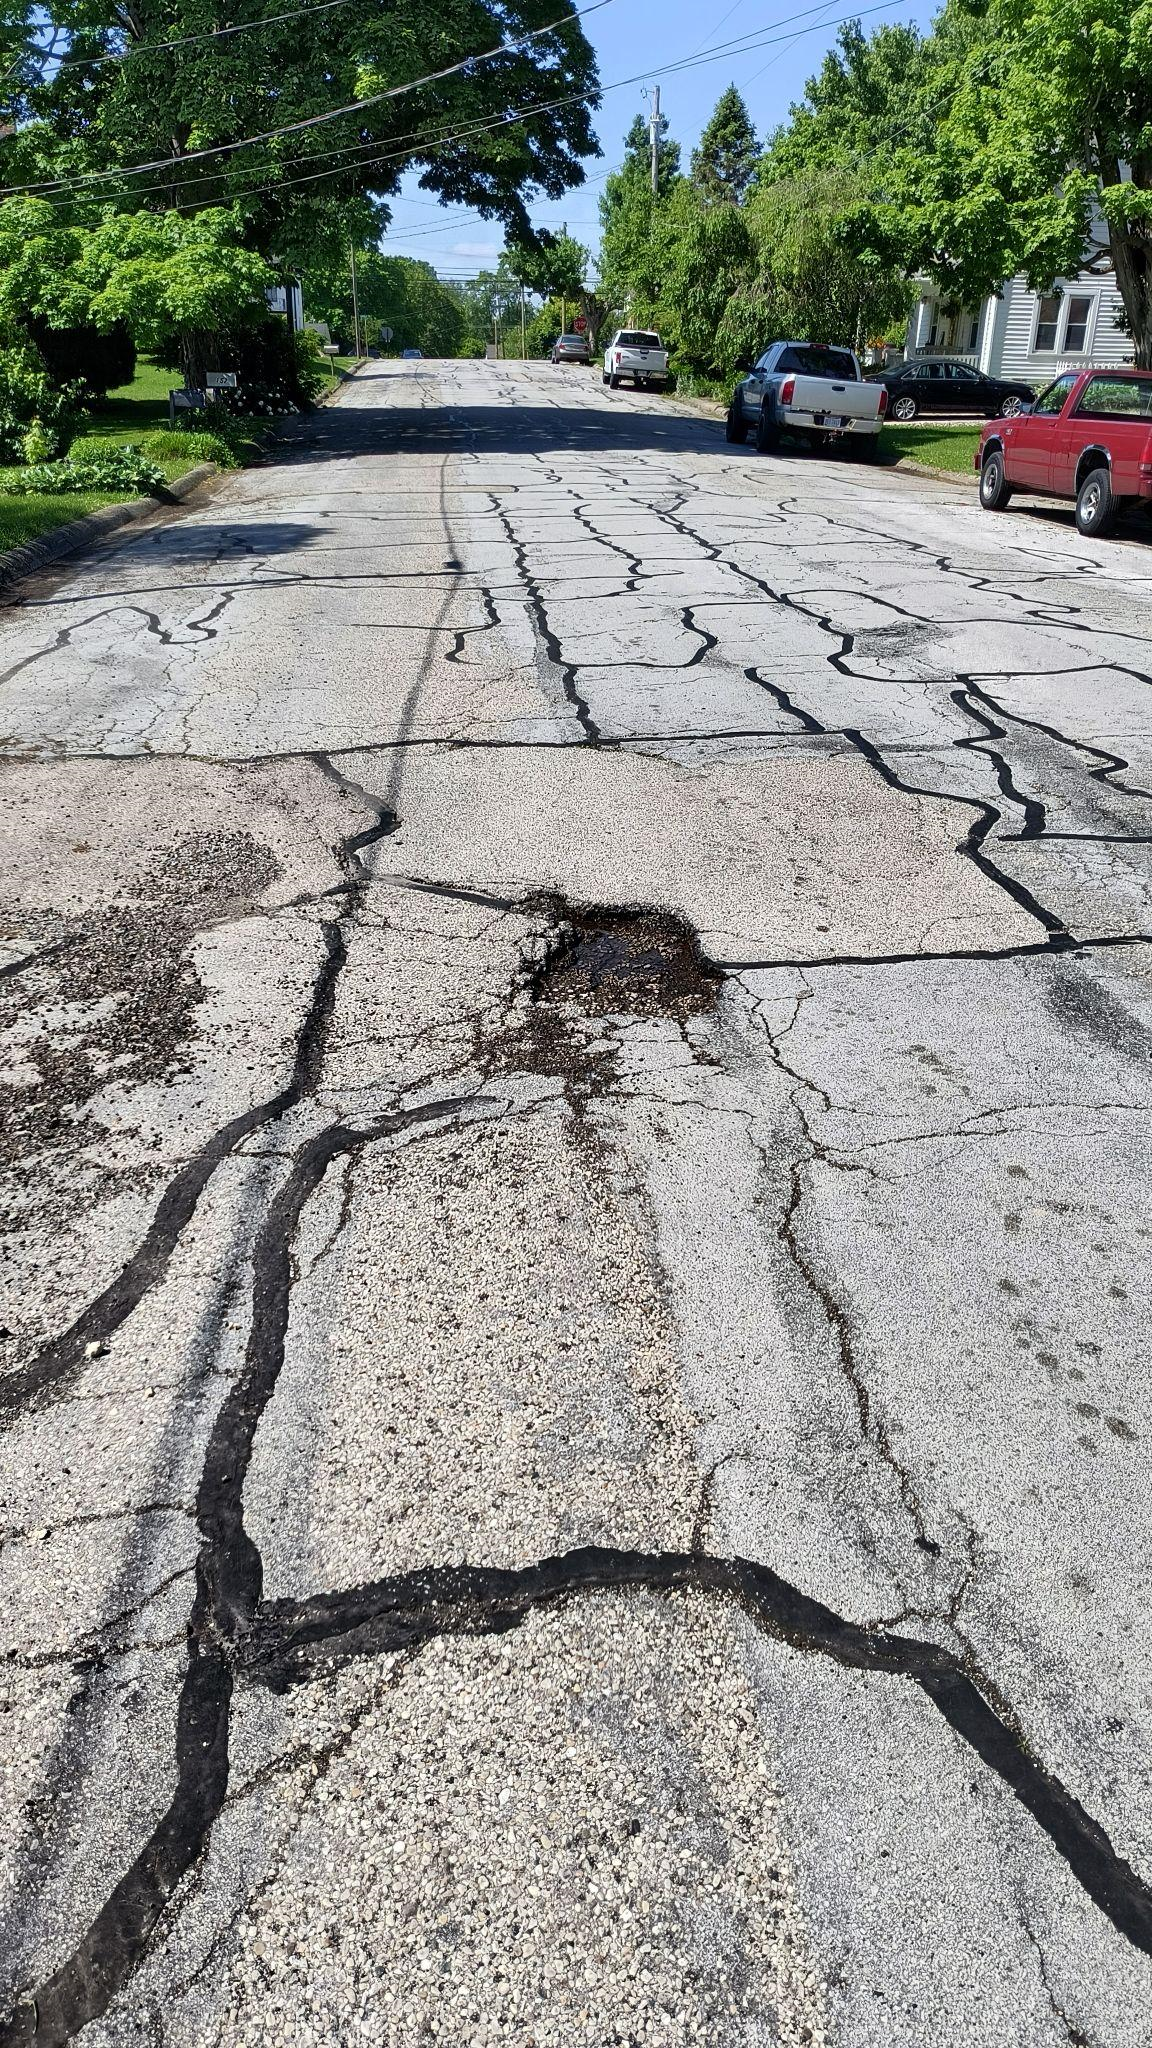
\includegraphics[width=0.75\textwidth,keepaspectratio]{images/waynesville_oh_1.png}
%         \caption*{Waynesville Road Image 1}
%         \label{fig:w_oh_1}
%     \end{minipage}
%     \hfill
%     \begin{minipage}[b]{0.48\textwidth}
%         \centering
%         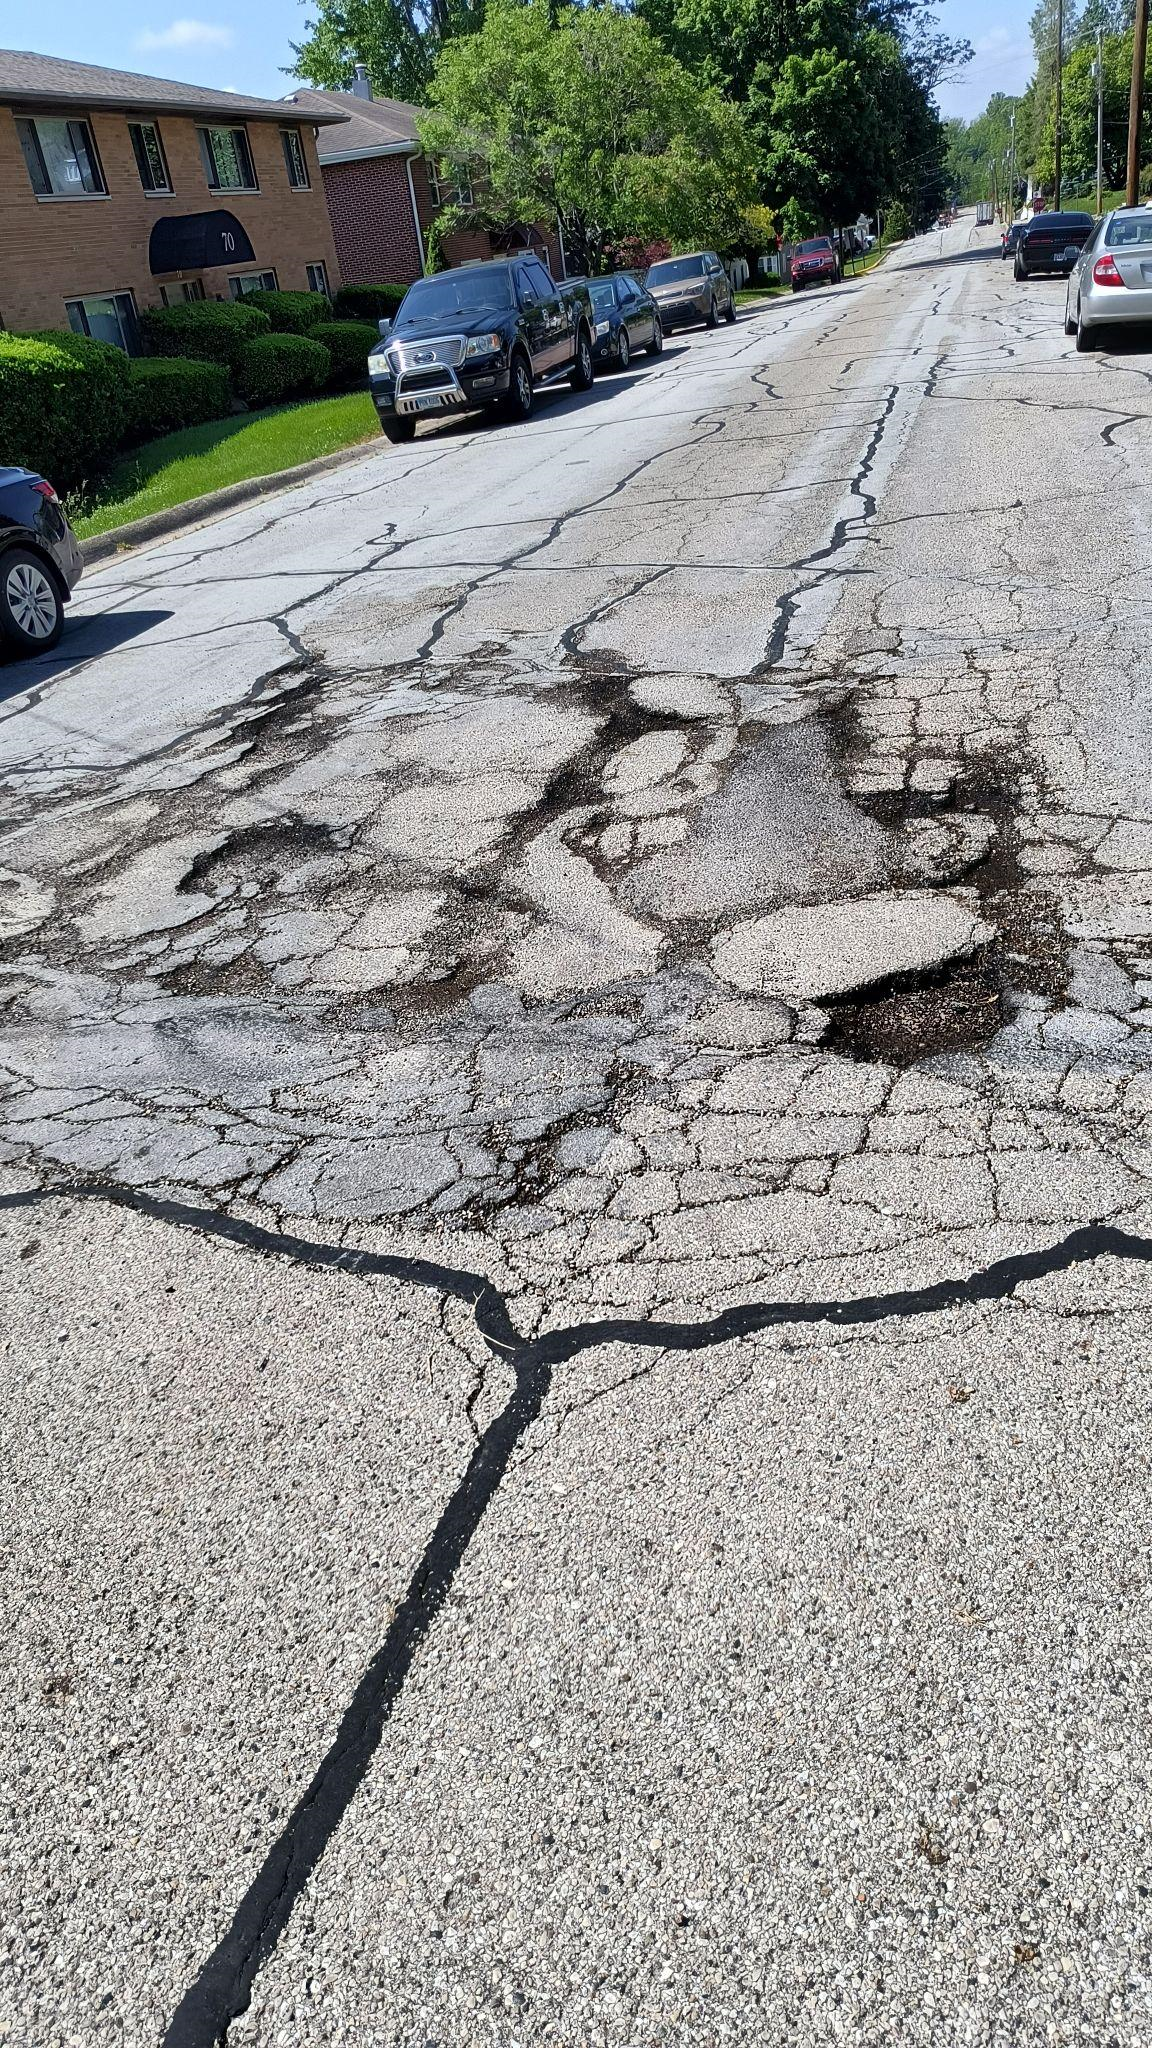
\includegraphics[width=0.75\textwidth,keepaspectratio]{images/waynesville_oh_2.png}
%         \caption*{Waynesville Road Image 2}
%         \label{fig:w_oh_2}
%     \end{minipage}

%     \vspace{1em}

%     \begin{minipage}[b]{0.48\textwidth}
%         \centering
%         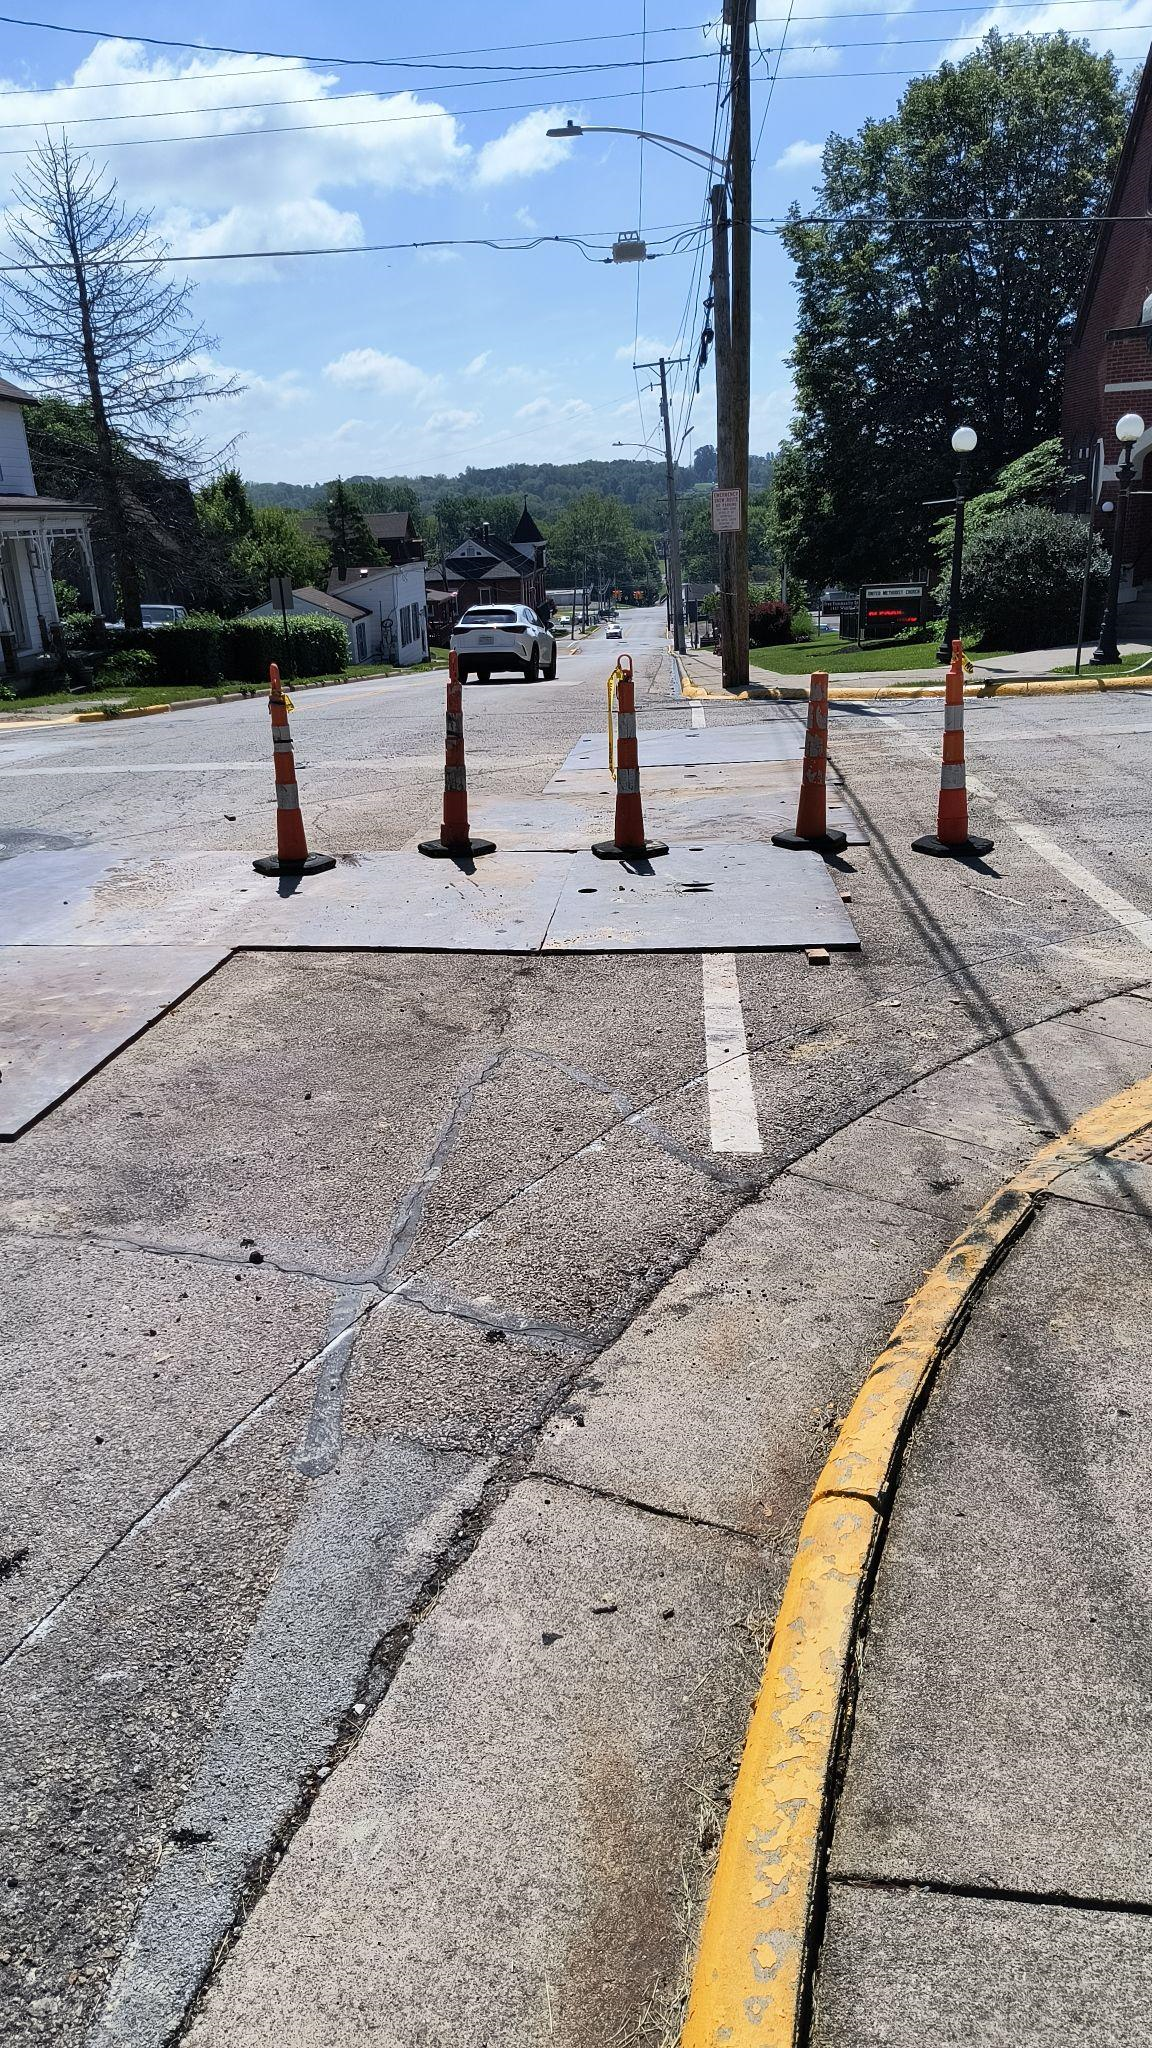
\includegraphics[width=0.75\textwidth,keepaspectratio]{images/waynesville_oh_3.png}
%         \caption*{Waynesville Road Image 3}
%         \label{fig:w_oh_3}
%     \end{minipage}

%     \caption{Roads in Waynesville: Case Study}
%     \label{fig:rd_waynesville}
% \end{figure}

% \section{More Details on Predicting Road Quality} \label{sec:appxd}




\clearpage

% \onehalfspacing

% \section*{Tables} \label{sec:tab}
% \addcontentsline{toc}{section}{Tables}


% \section*{Figures} \label{sec:fig}
% \addcontentsline{toc}{section}{Figures}

%\begin{figure}[hp]
%  \centering
%  \includegraphics[width=.6\textwidth]{../fig/placeholder.pdf}
%  \caption{Placeholder}
%  \label{fig:placeholder}
%\end{figure}




\clearpage

% \section*{Appendix A. Placeholder} \label{sec:appendixa}
% \addcontentsline{toc}{section}{Appendix A}



\end{document}